\documentclass[12pt,oneside,bibtotoc,liststotoc]{scrbook}
\usepackage[utf8]{inputenc}
\usepackage{graphicx}
\usepackage{float}
\usepackage[ngerman,english]{babel}
\usepackage{a4wide}
\usepackage{parskip}
\usepackage[bookmarks]{hyperref}
\usepackage{fancyhdr}
\usepackage[right]{eurosym}
\usepackage{amsmath}
\usepackage{amsfonts}
\usepackage[toc,page]{appendix}

\usepackage[numbers]{natbib}
\DeclareUnicodeCharacter{2192}{ to}

\usepackage{lstautogobble}

\usepackage{array}
\usepackage{longtable}
\usepackage{booktabs}
\usepackage{listings}
\usepackage{color}
\usepackage[usenames,dvipsnames]{xcolor}
\colorlet{punct}{red!60!black}
\definecolor{background}{HTML}{EEEEEE}
\definecolor{delim}{RGB}{20,105,176}
\colorlet{numb}{magenta!60!black}
\lstdefinelanguage{json}{
    basicstyle=\footnotesize\ttfamily,
    numbers=left,
    tabsize=2,
    lineskip={-1.0pt},
    numberstyle=\scriptsize,
    stepnumber=1,
    numbersep=8pt,
    showstringspaces=false,
    breaklines=true,
    frame=lines,
    backgroundcolor=\color{background},
    literate=
      *{:}{{{\color{punct}{:}}}}{1}
      {,}{{{\color{punct}{,}}}}{1}
      {\{}{{{\color{delim}{\{}}}}{1}
      {\}}{{{\color{delim}{\}}}}}{1}
      {[}{{{\color{delim}{[}}}}{1}
      {]}{{{\color{delim}{]}}}}{1},
}
\lstdefinelanguage{rdf}{
    basicstyle={\footnotesize\ttfamily},
    lineskip={-1.0pt},
    numbers=left,
    numberstyle=\scriptsize,
    stepnumber=1,
    numbersep=8pt,
    showstringspaces=false,
    breaklines=true,
    frame=lines,
    tabsize=2,
    backgroundcolor=\color{background},
    keywordstyle={\bfseries\color{Blue}},
    commentstyle={\color{Red}\textit},
    stringstyle=\color{Magenta},
    morekeywords={ql,rml,rr,schema},
    moredelim=*[s][\ttfamily]{:}{:} %Newly added line
}
\lstdefinelanguage{xml}{
    basicstyle={\footnotesize\ttfamily},
    lineskip={-1.0pt},
    numbers=left,
    tabsize=2,
    numberstyle=\scriptsize,
    stepnumber=1,
    numbersep=8pt,
    showstringspaces=false,
    breaklines=true,
    frame=lines,
    backgroundcolor=\color{background},
    keywordstyle={\bfseries\color{Blue}},
    commentstyle={\color{Red}\textit},
    stringstyle=\color{Magenta},
    morekeywords={ServiceProvider,Document,Address,Service,Product,Occupancy,Price},
    moredelim=*[s][\ttfamily]{:}{:} %Newly added line
}
\newcommand\tab[1][1cm]{\hspace*{#1}}
\lstset{
	basicstyle=\ttfamily\small,
	showspaces=false,
	numbers=left,
	breaklines = true,
	showstringspaces=false
}

\pagestyle{headings}
\setlength{\textwidth}{15cm}
\setlength{\textheight}{22.5cm}
\setlength{\oddsidemargin}{1cm}
\setlength{\evensidemargin}{0cm}
\begin{document}

\thispagestyle{empty}
\begin{center}
\LARGE{Leopold-Franzens Universität Innsbruck\\ Faculty of Mathematics, Computer Science and Physics}\\[3ex] \large{Department of Computer Science}\\[2ex]
\end{center}
\medskip

\begin{center}

\includegraphics[width=3cm]{Logo}
\vspace{1cm}

\textbf{\LARGE{Bachelor’s Thesis}} \medskip\par \textbf{\normalsize{submitted for the degree of}} \\[3ex] \textbf{\Large{Bachelor of Science}}
\vspace{1.5cm}

\textbf{\Large{Symbolic Regression for Surrogate Modeling - A Systematic Study}} \bigskip\par von \par \large{Tobias Albrecht}\\ (Matr.-Nr.: 12206456)
\end{center}
\vspace{1cm}

\begin{tabular}{ll}
  Submission Date:  & \textcolor{red}{TODO: Add Submission Date} \\
  Supervisor: & Ass.-Prof. Philipp Zech, PhD \\
\end{tabular}

\newpage

\vspace*{5cm}

\begin{center}
\LARGE{Eidesstattliche Erklärung}\\
\end{center}
\vspace{1cm}


\begin{quote}
\emph{Ich erkläre hiermit an Eides statt durch meine eigenhändige Unterschrift, dass ich die vorliegende Arbeit selbstständig verfasst und keine anderen als die angegebenen Quellen und Hilfsmittel verwendet habe. Alle Stellen, die wörtlich oder inhaltlich den angegebenen Quellen entnommen wurden, sind als solche kenntlich gemacht. \\Ich erkläre mich mit der Archivierung der vorliegenden Bachelorarbeit einverstanden. }
\end{quote}
\vspace{2.5cm}

\begin{flushleft}
\begin{tabular}{lll}
Ort und Datum: & & \rule{7cm}{0.4pt}\\[7ex]
Unterschrift: & & \rule{7cm}{0.4pt}
\end{tabular}
\end{flushleft}

\thispagestyle{empty}

\newpage

\vspace*{5cm}

\begin{center}
\LARGE{Disclaimer on the Use of AI}\\
\end{center}
\vspace{1cm}


\begin{quote}
\emph{\textcolor{red}{TODO: Add Disclaimer on the Use of AI}}
\end{quote}
\vspace{2.5cm}

\thispagestyle{empty}

\renewcommand{\baselinestretch}{1.00}\normalsize

\setcounter{page}{1}
\pagenumbering{Roman}

\chapter*{Abstract}
\addcontentsline{toc}{chapter}{Abstract}

Surrogate models are often used in scientific and engineering applications to approximate computationally expensive simulations. However, many flexible surrogate methods produce black-box models whose learned relationships are difficult to inspect. Symbolic Regression (SR) addresses this limitation by discovering explicit mathematical expressions directly from data, thereby combining predictive modeling with an inspectable model representation.

This thesis provides a systematic study of Symbolic Regression methods for surrogate modeling. The main goal is to compare open-source SR frameworks that employ different algorithmic approaches, including evolutionary, genetic programming, transformation-based, and neural methods. The evaluated frameworks are gplearn, Operon, PySR, GeneticEngine, ITEA, and EQL.

To evaluate these frameworks, the benchmark uses ten problems from different domains, including engineering, physics, materials, energy systems, building simulation, and aeroacoustics. The selected SR models are evaluated using identical training and test data and a common evaluation protocol with documented algorithm-specific search budgets. The evaluation considers predictive accuracy, computational efficiency, model complexity, stability across repeated trials, sensitivity to input scaling, and practical usability. The thesis also investigates the trade-offs between accuracy and interpretability, as well as current challenges in Symbolic Regression for surrogate modeling.

Across 1200 planned trials, 1199 completed successfully. Operon achieved the lowest mean range-normalized RMSE in 13 of 20 problem--scaling combinations, the best median value of 0.0259, and the shortest median fitting time of 3.88 seconds. PySR produced the smallest expressions, ITEA offered a strong balance of accuracy, runtime, and compactness, and EQL benefited most consistently from input normalization. The results show that SR can provide inexpensive and inspectable surrogates, but suitability depends on the problem and objective, and predictive success does not guarantee a simple, stable, or scientifically meaningful model.

\tableofcontents
\listoffigures
\listoftables
% \renewcommand{\baselinestretch}{1.5}\normalsize
\newpage
\setcounter{page}{1}
\pagenumbering{arabic}

\chapter{Introduction}

Scientific and engineering research mostly relies on numerical simulations and physical experiments to investigate complex systems, optimize technical designs, and evaluate control strategies. High-fidelity simulations may require expensive numerical solvers, while physical experiments may be time consuming and costly. These costs become a practical bottleneck when a system must be evaluated repeatedly, for example during optimization, uncertainty quantification, sensitivity analysis, or parameter exploration \cite{alizadeh2020managing}.

A surrogate model is trained on observations obtained from simulations, physical measurements, or both and is then used to provide inexpensive predictions for new inputs. This approach is widely used to manage computational complexity in engineering design and simulation-based analysis, where the cost of generating training data must be balanced against predictive accuracy and the computational savings achieved during repeated evaluation \cite{alizadeh2020managing}. Surrogate models are particularly useful in domains such as physics, mechanical engineering, materials science and energy systems, where obtaining direct simulation results or experimental measurements can be expensive.

Modern machine learning methods are common choices for surrogate modeling because they can approximate complex nonlinear relationships. Neural networks, ensemble models, Gaussian processes, and other flexible approaches achieve strong predictive performance \cite{alizadeh2020managing}. However, this flexibility can make the resulting surrogate difficult to inspect, explain, or compare with known scientific relationships. This lack of transparency may be acceptable when a surrogate is used only for prediction. However, when the model is intended to support scientific understanding, engineering decisions, or safety-relevant applications, predictive accuracy alone may be insufficient, and the structure and behavior of the learned model must also be considered.

\section{The Need for Interpretable Models}

Interpretability becomes important when a model is intended to support scientific understanding rather than prediction alone. In scientific and engineering applications, an interpretable surrogate can help researchers inspect which variables appear in the learned relationship, examine their nonlinear interactions, and compare the model structure with established domain knowledge. These forms of inspection are difficult when the surrogate is a black box since a low prediction error on testing data does not by itself demonstrate that a model has learned a scientifically meaningful or domain-consistent relationship.

% This issue is especially relevant when surrogate models are used outside the exact setting in which they were trained. A model can perform well on a test set but still produce unrealistic predictions on unseen input ranges, react poorly to noisy input, or accumulate prediction errors when used iteratively. Interpretable models provide additional ways to evaluate this behavior. Their structure can be inspected, simplified, checked against domain knowledge, and analyzed for physical plausibility.

The distinction between interpretable models and post-hoc explanations is important. Rudin argues that in high-stakes settings, one should prefer models that are interpretable by design instead of first training a black-box model and then trying to explain it afterward \cite{rudin2019stop}. This argument is also relevant for scientific surrogate modeling. If the learned model is meant to support reasoning about a physical or engineering system, the transparency of the model itself is important.

Interpretability is not a single property. A model may be considered interpretable because it is simple, because it uses familiar mathematical operations or because its variables have clear roles. In surrogate modeling, interpretability also must be balanced against accuracy. A very simple model may be easy to understand but too inaccurate to be useful, while a highly accurate model may be too complex to provide valuable insight. This trade-off motivates benchmarking the different frameworks according to both predictive accuracy and model complexity \cite{lacava2021contemporary,defranca2025srbench}.

\section{Symbolic Regression as a Candidate Approach}

Symbolic Regression (SR) is a machine learning approach that searches for explicit mathematical expressions fitting a given dataset. Instead of assuming a fixed model form, such as a linear model or a predefined polynomial basis, SR explores combinations of variables, constants, and mathematical operators. The result is not only a predictor but also an equation that can be read, evaluated, simplified, and compared with domain knowledge \cite{makke2024interpretable,dong2025recent}.

This makes SR a promising candidate for interpretable surrogate modeling. A symbolic expression can often be much cheaper to evaluate than the original simulation and more transparent than the black-box models. SR has therefore received considerable attention in scientific discovery, including physics, materials science, and dynamical systems \cite{angelis2023artificial,guo2024harnessing,wang2024exploring,brum2026discovering}.

Several well-known examples illustrate the scientific motivation for SR. AI Feynman uses physics-inspired strategies to recover equations from the Feynman Lectures on Physics, showing how prior structural ideas such as symmetry and separability can support symbolic equation discovery \cite{udrescu2020ai}. Sparse Identification of Nonlinear Dynamics (SINDy) similarly pursues interpretable governing equations from data, although it uses sparse regression over a predefined library of candidate terms rather than general symbolic search \cite{brunton2016discovering}. These works show the broader appeal of data-driven equation discovery for scientific modeling.

At the same time, SR is not automatically superior to other surrogate modeling approaches. The search space of possible expressions is large, and different frameworks use different strategies to explore it. Evolutionary algorithms, genetic programming variants, and neural or reinforcement-learning-based approaches differ in their assumptions, computational cost, ease of use, and ability to discover compact expressions \cite{dong2025recent,petersen2021deep}. The quality of the final model also depends on operator choices, complexity penalties, training budgets, and implementation details.

\section{Research Question and Contributions}

The central research question of this thesis is:

\begin{quote}
\emph{How suitable are Symbolic Regression frameworks for interpretable surrogate modeling, and how do they compare with respect to predictive performance, computational cost, equation complexity, and practical usability?}
\end{quote}

To answer this question, this thesis conducts a systematic study of six open-source SR frameworks: gplearn \cite{stephens2026gplearn}, Operon \cite{burlacu2020operon}, PySR \cite{cranmer2023interpretable}, GeneticEngine \cite{espada2022datatypes}, ITEA \cite{defranca2021itea}, and EQL \cite{sahoo2018eql}. The selected frameworks represent different approaches to symbolic model discovery, including tree-based genetic programming, efficient evolutionary search, grammar-guided genetic programming, interaction transformation based evolutionary search, and neural equation learning. The frameworks are evaluated on ten analytical, simulator-generated, experimental, and measured surrogate-modeling problems using fixed training and test datasets and documented algorithm-specific search budgets. The comparison considers predictive accuracy, computational efficiency, expression complexity, stability across repeated trials, sensitivity to input scaling, practical usability, and reproducibility.

The main contributions of this thesis are:

\begin{itemize}
    \item a structured overview of Symbolic Regression as an approach for interpretable surrogate modeling;
    \item a benchmark setup for comparing the selected SR frameworks on datasets from different application domains;
    \item an evaluation protocol covering predictive accuracy, runtime, equation complexity, stability across repeated fitting trials, and qualitative practical usability;
    \item an interpretability-oriented comparison of the discovered symbolic expressions;
    \item practical guidance on strengths, limitations, and challenges of the current SR frameworks for surrogate modeling.
\end{itemize}

The remainder of this thesis is organized as follows. Chapter 2 introduces the background on surrogate modeling, Symbolic Regression, method families, and interpretability. Chapter 3 discusses related work, including existing reviews, benchmark studies, and applications. Chapter 4 describes the methodology, including framework and dataset selection, evaluation metrics, reproducibility setup, and interpretability. Chapter 5 presents the experimental setup. Chapter 6 reports the results. Chapter 7 discusses the findings and their limitations. Chapter 8 concludes the thesis and outlines directions for future work.


\chapter{Background}

This chapter introduces the theoretical background of the thesis. It discusses surrogate modeling, the role of interpretable models, the foundations and challenges of Symbolic Regression, and the frameworks selected for the benchmark.

\section{Surrogate Modeling}

Many scientific and engineering workflows rely on simulation models that provide detailed representations of physical systems but are computationally expensive to evaluate. Finite element analysis and computational fluid dynamics are prominent examples. Their computational cost becomes a practical limitation when numerous evaluations are required for tasks such as design optimization, uncertainty quantification, sensitivity analysis, or exploration of a parameter space \cite{alizadeh2020managing}.

A surrogate model approximates the input output relationship of the computationally expensive simulation or physical process. It is constructed from a finite set of observations and is intended to provide predictions at a substantially lower evaluation cost than the original process \cite{alizadeh2020managing}. If the original model is denoted by

\begin{equation}
    y = f(\mathbf{x}),
\end{equation}

where $\mathbf{x} \in \mathbb{R}^{d}$ is an input vector and $y \in \mathbb{R}$ is the corresponding output, a surrogate model approximates this relationship with a function $\hat{f}$ such that

\begin{equation}
    \hat{y} = \hat{f}(\mathbf{x}) \approx f(\mathbf{x}).
\end{equation}

The main practical advantage of a surrogate is that evaluating $\hat{f}$ is generally less computationally expensive than evaluating the original model $f$. This makes repeated model evaluations feasible, but computational efficiency alone does not determine whether a surrogate is useful. Its predictive accuracy on relevant unseen data, the amount of data required for its construction, and the computational cost of fitting and evaluating it must also be considered \cite{alizadeh2020managing}.

A wide range of statistical and machine-learning methods can be employed as surrogate models, including polynomial response surfaces, Gaussian processes, artificial neural networks, support vector regression, boosted trees, and random forests \cite{alizadeh2020managing}. These methods can approximate complex nonlinear relationships without requiring a complete analytical description of the underlying process. However, flexible predictive models may provide limited insight into the learned input output relationship \cite{makke2024interpretable}.

\section{Symbolic Regression}

Symbolic Regression (SR) is a supervised learning approach that searches for mathematical expressions fitting a given dataset. In contrast to ordinary regression methods, SR does not assume a fixed functional form in advance. For example, a linear regression model assumes that the target can be represented as a weighted sum of input variables. A polynomial regression model assumes a predefined set of polynomial terms. SR instead searches over both the structure of the expression and its numerical parameters \cite{angelis2023artificial,lacava2021contemporary}.

Symbolic regression (SR) searches for a mathematical expression that describes the relationship between input variables and a target variable directly from data \cite{makke2024interpretable}. Consider a supervised dataset

\begin{equation}
    D = \{(\mathbf{x}_i, y_i)\}_{i=1}^{N},
\end{equation}

where $D$ denotes the complete dataset, $N$ is the number of observations, and $i \in \{1,\ldots,N\}$ indexes an individual observation. The vector $\mathbf{x}_i \in \mathbb{R}^{d}$ contains the values of the $d$ input variables for the $i$-th observation, while $y_i \in \mathbb{R}$ is its corresponding target value.

Symbolic Regression can be divided into Explicit Symbolic Regression (ESR) and Implicit Symbolic Regression (ISR). ESR searches for a function that expresses a designated target directly in terms of the input variables, such as $y=\phi(\mathbf{x};\boldsymbol{\theta})$. ISR instead searches for a relation of the form $F(\mathbf{x},y;\boldsymbol{\theta})=0$, without requiring one variable to be isolated as the target. This thesis considers ESR because all benchmark problems define a continuous target that must be predicted from a given set of input variables \cite{dong2025recent}.

The objective of ESR in this thesis is to find both a symbolic expression structure $\phi$ and numerical constants $\boldsymbol{\theta}$ such that the prediction $\phi(\mathbf{x}_i;\boldsymbol{\theta})$ approximates $y_i$. For example, one possible measure of prediction error is the mean squared error (MSE),

\begin{equation}
    \mathcal{L}_{\mathrm{MSE}}(\phi,\boldsymbol{\theta})
    =
    \frac{1}{N}
    \sum_{i=1}^{N}
    \left(
        y_i - \phi(\mathbf{x}_i;\boldsymbol{\theta})
    \right)^2.
\end{equation}

where $y_i - \phi(\mathbf{x}_i;\boldsymbol{\theta})$ denotes the prediction error for the $i$-th observation.

However, minimizing prediction error alone can produce unnecessarily large expressions. Because the result of SR is intended to remain interpretable, expression complexity must also be considered. Complexity may, for example, be measured by the number of nodes or operators in the expression tree. SR is therefore commonly treated as a multi objective problem involving a trade-off between predictive accuracy and expression complexity \cite{cranmer2023interpretable,lacava2021contemporary}.

Candidate expressions are commonly represented as syntax trees. In such a tree, internal nodes are mathematical operators such as $+$, $-$, $\times$, division, $\sin$, $\cos$, $\log$, or $\exp$, while leaf nodes are variables or constants. For example, the expression

\begin{equation}
    \phi(x_1,x_2) = 3 x_1 + \sin(x_2 / 5)
\end{equation}

can be represented as a tree combining multiplication, division, addition, two constants, two variables, and a sine operator.

\textcolor{red}{TODO: Add an actual tree diagram.}

This representation makes it possible to modify expressions by changing subtrees, replacing operators, or adjusting constants.

The search space of SR is very large. Even a small set of variables and operators can generate many possible expressions, and the number of possible expressions grows quickly with expression size. This is one reason why SR is computationally difficult and why many frameworks use different search strategies \cite{dong2025recent}. Another challenge is the treatment of constants. In scientific equations, real-valued constants are often essential, but searching simultaneously over expression structure and continuous constants is much harder than fitting coefficients in a fixed model form \cite{cranmer2023interpretable}.

Despite these challenges, SR is useful for scientific modeling because its outputs can be interpreted directly. A discovered equation can be evaluated cheaply, simplified symbolically, compared with existing theory, inspected for asymptotic behavior, and checked for physically implausible terms. This distinguishes SR from many black-box methods, where interpretability is usually added after training through explanation methods rather than being part of the model itself \cite{makke2024interpretable}.

\section{Main Symbolic Regression Method Families}

Recent surveys group SR methods into several broad families. The most relevant distinction for this thesis is between deterministic methods, genetic programming methods, and neural methods \cite{dong2025recent}. These families differ in how they explore the expression space and handle constants.

\textcolor{red}{TODO: Ask if this is needed.}

The distinction between Explicit and Implicit Symbolic Regression is separate from this classification by method family. ESR and ISR describe the form of the relationship being discovered, whereas deterministic, genetic programming, and neural methods describe how the expression space is searched. Methods from these families can therefore be developed for either explicit or implicit relationships. However, all frameworks evaluated in this thesis perform ESR because they construct an explicit prediction of a designated target variable from the given inputs.

Deterministic methods use systematic search, enumeration, sparse regression, mixed-integer optimization, or related strategies to explore candidate expressions. Their main advantage is that they can be more stable and reproducible than purely stochastic methods, because the search process is less dependent on random initialization. Some deterministic approaches can also provide stronger guarantees within a restricted search space. The limitation is that the number of possible expressions grows rapidly with the number of variables, operators, and expression depth. As a result, deterministic methods may become computationally expensive for high-dimensional or complex problems \cite{dong2025recent}.

Genetic Programming (GP) methods are historically the most established family of SR algorithms. GP treats expressions as individuals in a population and evolves them over many generations. Candidate expressions are evaluated according to a fitness function, selected, recombined, mutated, and simplified. This family is flexible because it can search over many different expression structures without requiring a fixed basis. It also naturally supports multi-objective optimization, where accuracy and complexity are optimized together \cite{angelis2023artificial,lacava2021contemporary}.

Neural-network-based SR methods use differentiable architectures or learned search strategies to construct mathematical expressions. The Equation Learner (EQL) evaluated in this thesis represents expressions using a shallow neural network whose units implement mathematical operations such as identity, multiplication, and trigonometric functions \cite{sahoo2018eql}. Its numerical parameters are optimized through gradient-based training, while sparsity regularization encourages the removal of unnecessary connections and allows the trained network to be converted into an explicit equation. EQL therefore performs ESR through a neural and differentiable model structure rather than through population-based evolution. Limitations of this approach include sensitivity to input scaling, optimization settings, and the set of mathematical operations built into the architecture.

The variety of method families is important for this thesis because there is no single best SR approach. A framework that performs well on one type of problem may behave differently on datasets with noise, high-dimensional inputs, or differently scaled variables. The comparison therefore treats the selected frameworks as explicit symbolic regression tools that share the same prediction objective but rely on different representations and search strategies.

\section{The Accuracy Complexity Trade-Off}

The central evaluation problem in SR is the trade-off between predictive accuracy and expression complexity. If only accuracy is optimized, SR can produce long expressions that fit the training data well but are difficult to interpret and prone to overfitting. If only simplicity is optimized, the resulting expression may be readable but too inaccurate to serve as a useful surrogate. A meaningful SR model should therefore achieve an appropriate balance between these objectives.

Complexity can be measured in different ways. A common syntactic measure is the number of nodes, operators, variables, and constants in an expression. Other measures consider expression depth, operator types, semantic behavior, nonlinearity, or the effective difficulty of understanding the formula \cite{lacava2021contemporary,dong2025recent}. There is no perfect complexity metric. A short equation can still be difficult to interpret if it contains unfamiliar or unstable operations, while a slightly longer equation may be more meaningful if it matches known domain structure.

Many SR frameworks return not only one expression but a set of candidate expressions along a Pareto front. A Pareto front contains models for which no other model is both more accurate and less complex. This is useful because the final choice of model depends on the application. For a deployment-focused surrogate, a slightly more complex expression may be acceptable if it improves predictions significantly. For scientific insight, a simpler expression may be preferable if it captures the dominant relation and remains physically plausible.

In this thesis, the accuracy complexity trade-off is treated as a core evaluation dimension. Predictive metrics such as mean squared error or coefficient of determination describe how well a model fits the data, while complexity metrics describe how complex the resulting expression is. Considering both dimensions is essential because a symbolic surrogate is only useful if it is accurate enough to approximate the underlying process and simple enough to support interpretation.

\section{Interpretability in Scientific Modeling}

Interpretability is a major motivation for applying SR to surrogate modeling. In scientific contexts, models are often expected to do more than predict. They should help explain a underlying system, reveal relationships between variables, and support reasoning about behavior in new conditions. A symbolic expression is attractive because the full mapping from inputs to outputs is visible in mathematical form.

The distinction between interpretability and post-hoc explainability is important. A black-box model may be explained after training using feature importance scores, saliency methods, local approximations, or other explanation techniques. These methods can be useful, but they do not make the original model transparent. An interpretable model, by contrast, exposes its structure directly. SR belongs to this second category, as it can produce sufficiently compact and meaningful expressions \cite{makke2024interpretable}.

SR can support scientific discovery when the resulting expression reveals a relation that was not explicitly provided to the model. Reviews of SR in physical sciences emphasize this potential. SR can generate analytical equations from data and thereby connect data-driven modeling with the traditional scientific practice of formulating laws and empirical relations \cite{angelis2023artificial,makke2024interpretable}. At the same time, interpretability should not be assumed automatically. A symbolic expression may be mathematically explicit but still too complex, unstable, or domain-inconsistent to be useful.

This thesis treats interpretability as an evaluation criterion rather than as a guaranteed outcome. The discovered expressions will be compared in terms of their size, structure, operator usage, and practical readability. This allows SR frameworks to be evaluated not only by whether they predict accurately, but also by whether they produce surrogate models that can plausibly support scientific understanding.


\chapter{Related Work}

The recent growth of Symbolic Regression (SR) has led to several survey papers that organize the field and summarize its main technical directions. Makke and Chawla provide a broad review of SR as a method for interpretable scientific discovery, emphasizing the ability of SR to infer compact mathematical expressions directly from data \cite{makke2024interpretable}. Their review discusses the historical development of SR, its relation to genetic programming, the emergence of deep-learning-based approaches, and applications in scientific domains. This perspective is closely aligned with the motivation of this thesis, because surrogate modeling in science and engineering often requires models that are not only accurate but also interpretable.

Angelis et al. focuses specifically on SR in the physical sciences \cite{angelis2023artificial}. Their review positions SR as a response to the limitations of black-box machine learning models in physics-based computation. They discuss SR as a data-driven method that can generate analytical equations and thereby support interpretation, generalization, and the discovery or verification of physical relations.

Dong and Zhong provide a more recent and comprehensive survey of advances in SR \cite{dong2025recent}. They organize SR methods into deterministic, genetic-programming-based, and neural-network-based families, and they also summarize benchmark datasets, evaluation metrics, software tools, and open research challenges. Their survey is useful for understanding the current methodological landscape and for motivating the framework selection in this thesis. In particular, the distinction between GP-based and neural SR approaches is relevant because the evaluated frameworks represent different search and implementation strategies.

These reviews show that SR is no longer limited to genetic programming. Current SR research includes evolutionary algorithms, deterministic search, sparse regression, reinforcement learning, transformer-based approaches, and hybrid methods. At the same time, the reviews also point to persistent challenges. For example, high computational cost, sensitivity to benchmark design, difficulty in evaluating interpretability, and inconsistent behavior across datasets.

\section{Benchmark Studies}

Benchmarking is a central issue in SR research because methods are often evaluated on different datasets, with different computational budgets, and with different definitions of success. Early SR papers frequently used small synthetic benchmarks, which made results difficult to compare across studies. Orzechowski, La Cava, and Moore addressed this issue by evaluating recent SR methods against standard machine learning regressors on a large set of regression problems \cite{orzechowski2018where}. Their study compared four GP-based SR methods with several scikit-learn regression methods on 94 real-world datasets. The results showed that SR methods can be competitive with strong machine learning baselines, but also that runtime remains as a limitation.

La Cava et al. extended this line of work with SRBench, a larger and more systematic benchmark for symbolic regression \cite{lacava2021contemporary}. SRBench compares 14 SR methods and 7 machine learning methods across 252 regression problems, including real-world datasets, ground-truth symbolic equations, physics equations, and systems of ordinary differential equations. Importantly, SRBench evaluates not only predictive accuracy but also expression complexity and symbolic solution recovery. The benchmark therefore provides a basis for comparing SR methods in terms of both predictive performance and expression complexity.

The SRBench results also highlight that no single method is universally optimal. Some frameworks perform strongly on black-box regression tasks, while others are better at recovering exact equations under controlled conditions. Operon, for example, is reported as one of the strongest methods on real-world black-box regression problems and as part of the best accuracy-simplicity trade-offs \cite{lacava2021contemporary}. These findings motivate a more focused comparison of selected frameworks in the surrogate modeling context, where practical usability, and interpretability are important.

More recent work has extended and criticized existing benchmark practices. SRBench++ argues that expression size alone is an insufficient proxy for interpretability and introduces domain-expert interpretation into the benchmarking process \cite{defranca2025srbench}. It also evaluates SR algorithms on more specific task properties, such as feature selection, robustness, extrapolation, and local minima. This is important because a symbolic expression can be short but still scientifically unhelpful, or slightly longer but more meaningful to a domain expert.

Aldeia et al. present a call for the next generation of SR benchmarks, arguing that SRBench should evolve as a living benchmark \cite{aldeia2025call}. Their work expands the set of evaluated methods, refines evaluation metrics, and considers trade-offs between accuracy, complexity, and energy consumption. The study emphasizes standardization of hyperparameter tuning, execution constraints, computational resources, and benchmark maintenance. These issues are directly relevant for this thesis because a fair comparison of SR frameworks requires a reproducible protocol.

Overall, benchmark studies show that SR evaluation is more complex than ordinary regression benchmarking. Accuracy, model complexity, solution recovery, runtime, robustness, and interpretability all matter. The present thesis builds on these insights but uses a narrower experimental scope. Instead of ranking many SR methods across hundreds of datasets, it compares a selected set of open-source frameworks under a reproducible surrogate modeling protocol.

\section{Selected Frameworks}

This thesis evaluates six open-source Symbolic Regression frameworks: gplearn, Operon, PySR, GeneticEngine, ITEA, and EQL. They were selected to represent different approaches to symbolic model construction, including conventional tree-based genetic programming, performance-oriented evolutionary search, grammar-guided genetic programming, interaction transformation expressions, and neural equation learning. The associated publications describe the algorithms and software architectures, while the exact versions and configurations used in this thesis are specified separately in the experimental methodology.

\subsubsection{gplearn}

Gplearn is a Python implementation of conventional tree-based genetic programming with an interface modeled after scikit-learn \cite{stephens2026gplearn}. Candidate expressions are represented as programs and evolved using tournament selection, crossover, and several forms of mutation, while a parsimony coefficient can be used to discourage unnecessarily large expressions. Unlike the other selected frameworks, gplearn does not have a dedicated peer-reviewed framework publication. However, it is included and characterized as a Koza-style symbolic-regression implementation in the SRBench comparison \cite{lacava2021contemporary}. Its comparatively direct implementation and familiar estimator interface make it a useful reference point for evaluating more specialized SR approaches.

\subsubsection{Operon}

Operon is an efficient C++ genetic programming framework designed specifically for Symbolic Regression \cite{burlacu2020operon}. It represents expression trees as contiguous linear sequences, which improves memory locality and enables efficient evaluation and manipulation of candidate models. Its modular evolutionary design is organized around offspring generators and supports automatic differentiation and gradient-based optimization of numerical constants. Operon emphasizes runtime performance, memory efficiency, and extensibility, making it relevant for examining how an optimized genetic programming implementation performs within the benchmark.

\subsubsection{PySR}

PySR is an open-source library for scientific Symbolic Regression that provides a Python interface to the Julia backend SymbolicRegression.jl \cite{cranmer2023interpretable}. Its search procedure uses multiple evolving populations and an evolve simplify optimize loop in which candidate expressions are evolved, simplified, and refined through numerical constant optimization. PySR also supports user defined operators, losses, complexity measures, and expression export to several scientific-computing formats. These capabilities make it a flexible framework to search for symbolic models under application specific mathematical constraints.

\subsubsection{GeneticEngine}

GeneticEngine is a Python framework for grammar-guided genetic programming in which the search space can be defined using Python data types rather than a separate textual grammar \cite{espada2022datatypes}. The framework combines ideas from grammar-guided and strongly typed genetic programming, allowing the structures and constraints of valid candidate programs to be expressed through the host language's type system. The publication emphasizes the ergonomics and expressive power of this representation and demonstrates this through an open source Python implementation.

\subsubsection{ITEA}

The Interaction Transformation Evolutionary Algorithm (ITEA) searches within a restricted representation in which models are formed as linear combinations of transformed interactions between input variables \cite{defranca2021itea}. Each interaction is defined through powers of the input variables and a selected transformation function, while the corresponding linear coefficients are fitted numerically. Rather than using conventional subtree crossover, ITEA evolves a population through mutation operations that add, remove, or modify terms, interactions, and transformations. This structured representation distinguishes ITEA from general expression-tree methods and provides direct control over the maximum number of terms in a model.

\subsubsection{EQL}

Equation Learning (EQL) represents mathematical expressions through a differentiable neural network whose units implement elementary operations such as identity, trigonometric functions, and multiplication \cite{sahoo2018eql}. Alternating linear transformations and operation-specific units allow the network to construct nonlinear analytical relationships, while sparsity regularization encourages a small number of active connections and therefore more concise expressions. The architecture is optimized using gradient-based methods rather than an evolutionary population, making EQL methodologically distinct from the other frameworks in the benchmark. The evaluated adapter implements the Equation Learner approach described in the associated literature.

The selected frameworks cover several parts of the contemporary SR landscape. gplearn, Operon, PySR, and GeneticEngine use different forms of genetic or evolutionary search, ITEA evolves expressions within the more restricted interaction transformation representation and EQL constructs equations through a differentiable neural architecture.


\chapter{Methodology}

This chapter describes the methodology used to design and conduct the benchmark. It presents the framework and dataset selection criteria, the common experimental protocol, the evaluation metrics, and the measures taken to ensure reproducibility.

\section{Framework Selection Criteria}

The purpose of this benchmark is not to identify a universally best Symbolic Regression algorithm, but to compare representative frameworks under conditions relevant to surrogate modeling. Framework selection was guided by five criteria:

\begin{itemize}
    \item the method is described in a scientific publication or has detailed software documentation;
    \item an open-source implementation is publicly available;
    \item the implementation returns an explicit mathematical expression rather than predictions alone;
    \item the framework can be integrated into the common SRBench-derived evaluation pipeline;
    \item the framework contributes a relevant algorithmic or representational approach to the comparison.
\end{itemize}

Practical installability, compatibility with the evaluation interface, and reproducible execution were also considered because technical failures and unavailable model expressions affect the usefulness of a framework in practice. This reflects recommendations that SR benchmarks should consider reproducibility, complexity, and practical execution in addition to predictive accuracy \cite{defranca2025srbench,aldeia2025call}.

Based on these criteria, six frameworks were included: gplearn, Operon, PySR, GeneticEngine, ITEA, and EQL. Together, they provide a range of evolutionary, representation-based, and gradient-based approaches to Symbolic Regression. Their exact configurations and execution environments are described in Chapter~5.

\section{Dataset Selection Criteria}

The benchmark problems were selected to represent scientific and engineering surrogate-modeling tasks while remaining feasible for repeated Symbolic Regression searches. Each problem is required to have numerical input variables, a continuous target, clearly documented feature meanings and domains, and a reproducible data source or generating function. The available data also had to support disjoint training and test sets without categorical encoding, missing-value imputation, or extensive feature engineering.

The selection combines four analytical problems with six external datasets. Cantilever, Borehole, Piston, and Wing Weight provide controlled relationships of different structural forms. Combined Cycle Power Plant, Naval Propulsion, Gas Turbine NOx Emissions, Concrete Compressive Strength, Energy Efficiency, and Airfoil Self-Noise add simulator-generated, measured, or experimental relationships from several engineering domains. All ten problems are evaluated using the same predictive, computational, stability, and expression-structure criteria; the analytical generating equations are used to construct controlled datasets but are not used as reference expressions in the interpretability comparison.

The final set of ten problems covers several engineering domains, between three and ten input variables, different physical scales, and relationships of varying structural difficulty. The analytical problems include multiplication, division, integer and fractional powers, logarithms, square roots, and trigonometric terms, while the external datasets introduce measurement variation and relationships for which the benchmark does not assume a privileged symbolic form. This combination allows the frameworks to be assessed across controlled and application-oriented surrogate-modeling tasks. The exact problem definitions, sample sizes, data sources, and train--test construction procedures are presented in Chapter~5.

\section{Benchmark Protocol}

All experiments use a common evaluation pipeline derived from SRBench \cite{lacava2021contemporary,srbenchRepository}. Each problem has a fixed training table and a separate test table that are generated or selected before the algorithm repetitions are executed. Dataset construction uses documented problem specific seeds, whereas the repetition seed controls the symbolic regression algorithm where supported. Consequently, every framework and repetition receives identical observations, preventing variation in dataset sampling from being confused with variation in algorithm behavior. SHA-256 hashes of the uncompressed training and test tables are stored in each result to make this invariant auditable.

Every algorithm problem combination is evaluated under two input-scaling conditions. In the \texttt{raw} condition, the stored inputs are supplied to the estimator in their original physical units. In the \texttt{domain\_minmax} condition, each input $x_j$ with documented lower and upper bounds $l_j$ and $u_j$ is mapped to $[-1,1]$ according to

\begin{equation}
    z_j = 2\frac{x_j-l_j}{u_j-l_j}-1.
\end{equation}

The transformation uses fixed problem-domain bounds rather than statistics estimated from the training data, ensuring that it is identical across frameworks and repetitions and does not introduce test-data leakage. Target values are not scaled and remain in their original units under both conditions. Expressions learned from normalized inputs are transformed back to the original physical variables during symbolic post processing.

The final repetition protocol uses the predefined labels 2, 3, 5, 7, 11, 13, 17, 19, 23, and 29. These labels are passed to each estimator that exposes a supported random-seed parameter. The ITEA implementation does not expose such a parameter, so its ten executions are reported as uncontrolled repetitions rather than seed-controlled trials. With six algorithms, ten problems, two input-scaling conditions, and ten repetitions, the complete benchmark contains 1200 expected trials.

Each trial fits one model using the fixed training target and evaluates it exclusively on the corresponding held-out reference-test set. A successful result, an explicit execution failure, and an absent trial are treated as three separate states. Failure records retain the algorithm, problem, scaling condition, repetition label, and process exit status, while the summary tables report successful, failed, and missing trials separately. Failed or missing runs are therefore not silently excluded from the reported experiment coverage.

Each framework uses one explicitly documented configuration across the benchmark, no hyperparameter optimization is performed using the final test results. The configured search effort is expressed through algorithm-specific controls, such as population sizes, generations, evaluation limits, iterations, or time limits. These settings were selected to make repeated execution feasible and do not impose equal computational budgets across frameworks. Runtime comparisons therefore describe the evaluated configurations and must not be interpreted as equal compute comparisons or estimates of the frameworks best attainable performance.

Shared execution controls restrict benchmark containers to one thread. After fitting each model predicts the complete test set five times to obtain a more reliable estimate of prediction time. Model fitting, prediction, and expression extraction are timed within the running algorithm environment. Container startup, image retrieval, dataset generation, result serialization, and symbolic post-processing are excluded from the reported algorithm runtime.

Symbolic parsing, transformation to physical coordinates, simplification, and structural measurement are performed as separate post-processing steps. Each stage has an independent timeout and writes a versioned analysis record without modifying the original trial result. Separating expression analysis from model execution ensures that a parsing or simplification failure does not invalidate an otherwise successful training and prediction trial.

\section{Evaluation Metrics}

This section defines the metrics used to compare the benchmarked frameworks. The evaluation considers predictive performance, computational efficiency, and expression complexity to capture both the quality and practical characteristics of the resulting symbolic models.

\subsection{Predictive Performance}

Predictive performance is evaluated exclusively on the held-out reference-test set. For target values $y_i$, predictions $\hat{y}_i$, the test-set mean $\bar{y}$, and $n$ test observations, the benchmark reports mean absolute error (MAE), root mean squared error (RMSE), and the coefficient of determination ($R^2$):

\begin{align}
    \mathrm{MAE} &= \frac{1}{n}\sum_{i=1}^{n}\left|y_i-\hat{y}_i\right|,\\
    \mathrm{RMSE} &= \sqrt{\frac{1}{n}\sum_{i=1}^{n}\left(y_i-\hat{y}_i\right)^2},\\
    R^2 &= 1-\frac{\sum_{i=1}^{n}\left(y_i-\hat{y}_i\right)^2}{\sum_{i=1}^{n}\left(y_i-\bar{y}\right)^2}.
\end{align}

MAE measures the average absolute prediction error, whereas RMSE assigns greater weight to large errors. Both remain in the target's original unit because target values are not scaled. The coefficient of determination measures performance relative to prediction by the test-set mean and may be negative when a model performs worse than that reference. Because the target ranges differ substantially between problems, raw MAE and RMSE values are interpreted within each problem rather than ranked directly across the complete dataset collection.

To provide a dimensionless error measure, the benchmark additionally reports range-normalized RMSE:

\begin{equation}
    \mathrm{NRMSE}_{\mathrm{range}}=\frac{\mathrm{RMSE}}{\max_i(y_i)-\min_i(y_i)}.
\end{equation}

The normalization uses the range of the reference-test target and allows prediction errors to be interpreted relative to the observed target variation. It does not modify the target values supplied during model fitting or prediction. The maximum absolute prediction error is also retained in each individual trial record as an additional indicator of the largest observed test-set deviation.

\subsection{Computational Efficiency}

Computational efficiency is evaluated using wall-clock measurements. The benchmark records the duration of the complete estimator fitting call and the first prediction over the reference-test set. Prediction of the full test set is repeated five times, from which the mean, median, and sample standard deviation are calculated. The median duration is also divided by the number of test observations and reported in microseconds per sample. Expression extraction is timed separately, while symbolic post-processing, container startup, image retrieval, dataset generation, and result serialization are excluded from the algorithm runtime.

\subsection{Expression Complexity}

Every returned expression is parsed with SymPy to obtain framework-independent structural measures. These include expression-tree node count, tree depth, operator count and operator set, constant count, and the number and identity of variables used. The same measures are calculated after symbolic simplification where possible. The adapter-specific model-size value is retained for reference but is not used as the primary cross-framework complexity measure because its definition differs between adapters.

\subsection{Practical Usability}

Practical usability is evaluated qualitatively rather than reduced to a single numerical score. The assessment considers whether a framework can be executed in a documented environment, integrated through the common estimator interface, supplied with a controllable repetition seed, used to return both predictions and an explicit expression, and processed by the shared symbolic-analysis pipeline. Trial completion, expression availability, parsing coverage, dependency or API incompatibilities, and the need for adapter-specific compatibility handling provide observable evidence for this assessment.

This definition concerns the use of each framework within the benchmark workflow and does not attempt to measure general software quality or the effort required for every possible installation environment. Setup observations, pinned container requirements, unsupported seed controls, execution failures, and compatibility workarounds are therefore reported descriptively alongside the quantitative predictive, timing, stability, and complexity results. No framework is assigned a composite usability rank because the importance of these factors depends on the intended application and reproducibility requirements.

\section{Reproducibility Setup}

The benchmark is organized around separate components for dataset preparation, framework adapters, trial evaluation, symbolic analysis, and result aggregation. Versioned JSON files under \texttt{configs/} define the problem set, repetition labels, input-scaling conditions, shared execution controls, and algorithm-specific parameters. Runner scripts under \texttt{scripts/} execute individual trials or the complete experiment matrix. The resolved configuration, its cryptographic hash, and the parameters accepted by the estimator are recorded with each trial result.

Algorithm environments are isolated using the published SRBench container images. The image references are pinned by immutable SHA-256 digests in \texttt{containers/images.lock}, preventing a later image update from silently changing the execution environment. The host virtual environment is used for dataset preparation, experiment coordination, symbolic post-processing, aggregation, and automated tests. Shared execution controls restrict the algorithm containers to one thread, while supported estimators receive the configured repetition seed.

Dataset origin is recorded independently of the algorithm runs. Analytical datasets are generated from documented equations, domains, and fixed generation seeds. External datasets retain their source URLs, identifiers, selection procedures, and source-file hashes. Every trial additionally records hashes of the exact training and test tables it received, making it possible to verify that all frameworks were evaluated on identical observations.

Trial results are stored under \path{results/<problem>/<benchmark>/<input-scaling>/<algorithm>/} as JSON files indexed by repetition label. Symbolic parsing, coordinate transformation, simplification, and structural measurement write separate analysis sidecars so that post-processing does not modify the original trial record. Aggregate CSV files are generated from these stored artefacts and report successful, failed, and missing trials explicitly.

\section{Interpretability Evaluation}

The interpretability evaluation is restricted to properties of the returned symbolic representation that can be measured consistently across all frameworks. It therefore treats expression availability, parseability, structural complexity, and simplification behavior as observable indicators of inspectability. These indicators complement predictive performance but do not establish by themselves that an expression is understandable to a particular reader or scientifically meaningful.

\subsection{Structural Measures}

After conversion to a SymPy expression tree, the benchmark records the total node count, tree depth, operator count and operator set, constant count, and the number and identity of variables used. Node count includes operator, variable, and numerical-constant nodes. Tree depth is the longest number of edges from the expression root to a leaf, with an isolated variable or constant having depth zero. Operator count records the number of non-leaf nodes, while the operator set identifies the distinct operation types present in the tree. Constants are numerical atomic nodes, and variables are the free symbols occurring in the expression.

These measures are calculated both for the parsed expression and, when simplification succeeds, for its simplified form. The framework-specific model-size value is retained in the trial record for reference but is not used for the primary comparison because the adapters define model size differently. The cross-framework analysis instead uses the common SymPy-based measures, with simplified node count serving as the principal summary of syntactic expression size.

\subsection{Parsing and Simplification Policy}

The original expression string returned by each adapter remains unchanged in the trial result. A separate post-processing stage translates the prefix notation used by gplearn and the infix notation used by the other frameworks into SymPy. Expressions learned with domain-normalized inputs are then transformed into the original physical input variables before their primary structural measures are calculated. Parsing success and any parsing error are recorded explicitly, and a parsing failure leaves the predictive result valid but prevents framework-independent structural measurement.

For a parsed expression, the post-processing procedure considers the parsed form together with cancelled, factored, factorized-after-cancellation, and generally simplified candidates. The valid candidate with the smallest node count is selected, with textual length used to break ties. Symbolic stages are bounded by the configured timeout. If simplification fails or exceeds its resource limit, the parsed unsimplified expression and its structural measures are retained as a documented fallback. Simplified and fallback expressions are counted separately and are not silently combined in the primary simplified-complexity averages.

\subsection{Interpretive Scope}

Smaller and shallower expressions with fewer operations may be easier to inspect, but syntactic complexity is only a proxy for interpretability. The recorded statistics do not measure whether an equation is physically plausible, dimensionally consistent, familiar to a domain expert, or useful for scientific reasoning. The evaluation reported in this thesis does not compare learned expressions with the analytical equations used to generate the controlled datasets. Interpretability is therefore discussed through the observed representation and its structural statistics, together with predictive accuracy, rather than through a claim that the underlying relationship was rediscovered.

\chapter{Experiments}

This chapter describes the realization of the benchmark protocol introduced in the methodology chapter. It defines the experimental matrix, documents how the individual datasets were constructed, records the configurations used for the six symbolic regression frameworks, and explains the execution and symbolic post-processing procedures.

\section{Experimental Matrix and Task Roles}

The experimental matrix combines ten regression problems, six symbolic regression frameworks, two input-scaling conditions, and ten repetitions. This produces
\begin{equation}
    10 \times 6 \times 2 \times 10 = 1200
\end{equation}
distinct trial coordinates.

The benchmark problems were selected to fulfill complementary experimental roles rather than to form a homogeneous dataset collection. Four analytical problems permit controlled sampling from relationships with different mathematical structures. The remaining six problems are based on measured, experimental, or simulator-generated data and represent applied surrogate-modeling tasks from energy, propulsion, materials, building simulation, and aeroacoustics.

\begin{longtable}{p{2.9cm}p{2.5cm}rrp{4.4cm}}
\caption{Problems and their roles in the experimental matrix.}
\label{tab:experiment-matrix}\\
\hline
Problem & Data type & Inputs & Train/test & Experimental role \\
\hline
\endfirsthead
\hline
Problem & Data type & Inputs & Train/test & Experimental role \\
\hline
\endhead
Cantilever & Analytical & 5 & 400/4000 & Rational power-law relationship\\
Borehole & Analytical & 8 & 400/4000 & Higher-dimensional rational relationship\\
Piston & Analytical & 7 & 400/4000 & Nonlinear relationship containing a nested square root \\
Combined Cycle Power Plant & Measured & 4 & 400/4000 & Low-dimensional industrial energy dataset \\
Naval Propulsion & Simulator-generated & 3 & 400/4000 & Propulsion-system surrogate with correlated operating variables \\
Wing Weight & Analytical & 10 & 400/4000 & Higher-dimensional expression with fractional powers and a trigonometric term \\
Gas Turbine NOx & Measured & 9 & 400/4000 & Industrial-emissions prediction with a chronological train--test separation \\
Concrete Strength & Experimental & 8 & 400/592 & Material-property prediction with replicated experimental observations \\
Energy Efficiency & Simulator-generated & 8 & 400/368 & Building heating-load prediction over simulated designs \\
Airfoil Self-Noise & Experimental & 5 & 400/1103 & Aeroacoustic prediction from wind-tunnel measurements \\
\hline
\end{longtable}

The analytical tasks emphasize controlled approximation of relationships with known structural characteristics, whereas the external datasets emphasize predictive performance on simulator-generated, experimental, and measured surrogate-modeling problems. All problems are evaluated using the same predictive, computational, stability, and expression-structure measures.

\section{Dataset Construction}

\subsection{Common Construction Procedure}

All training and reference-test tables are constructed before the symbolic regression repetitions are executed. Dataset construction uses fixed problem-specific seeds that are independent of the framework repetition labels. The resulting tables are therefore identical for all frameworks and repetitions within a problem and input-scaling condition. SHA-256 hashes of the uncompressed tables are recorded in each trial result so that this property can be verified.

\subsection{Analytical Datasets}

The Cantilever problem is generated from its analytical rational power-law equation using five input variables. A single random generator is used to draw the 400 training observations followed by the 4000 reference-test observations.

The Borehole problem contains eight input variables and is generated from the standard analytical borehole-flow equation. The training and reference-test designs are independently generated using scrambled Latin hypercube sampling. The equation contains several nonlinear interactions, including logarithmic and rational terms, making it a more structurally demanding approximation task than the Cantilever problem.

The Piston problem contains seven inputs and represents the cycle time of a simulated piston system. Scrambled Latin hypercube designs are used for the training and reference-test tables. The generating expression contains multiple intermediate interactions and a nested square root, allowing the benchmark to examine whether the frameworks can approximate a comparatively deep analytical structure.

The Wing Weight problem contains ten inputs and is generated from an analytical aircraft-wing weight equation. Independent scrambled Latin hypercube samples produce the training and reference-test tables. The equation combines products, fractional powers, and a cosine term, thereby extending the analytical task collection beyond rational and square-root expressions.

\subsection{External Datasets}

The Combined Cycle Power Plant dataset is obtained from the UCI Machine Learning Repository and contains 9568 observations with four input variables. A fixed permutation is applied to the complete dataset. The first 400 permuted observations form the training set, and the following 4000 observations form the reference-test set.

The Naval Propulsion problem is based on the UCI Condition Based Maintenance of Naval Propulsion Plants dataset. The source data contains a full factorial simulator design with 11934 observations. Three operating variables are used to predict the selected propulsion-system target.

The Gas Turbine NOx problem is constructed from five annual UCI gas-turbine emissions files containing 36733 observations in total. Nine ambient and process variables are used to predict nitrogen-oxide emissions, while the year indicator and carbon-monoxide target are excluded.

The Concrete Strength problem is obtained from the UCI Concrete Compressive Strength dataset. Observations with identical values for all eight input variables are aggregated into distinct experimental designs, and their target values are combined, producing 992 unique designs.

The Energy Efficiency problem is obtained from the UCI Energy Efficiency dataset and contains 768 simulated building designs with eight input variables. Heating load is used as the target, while cooling load is excluded. A fixed permutation assigns the first 400 designs to the training set and the remaining 368 designs to the reference-test set.

The Airfoil Self-Noise problem is obtained from the UCI Airfoil Self-Noise dataset and contains 1503 wind-tunnel observations with five input variables. Scaled sound-pressure level is used as the target. A fixed permutation assigns 400 observations to the training set and the remaining 1103 observations to the reference-test set.

\subsection{Input Normalization}

For the domain-normalized condition, each raw input $x_j$ is transformed using the documented lower and upper bounds $l_j$ and $u_j$ of its problem domain:
\begin{equation}
    z_j = 2\frac{x_j-l_j}{u_j-l_j}-1.
    \label{eq:experiment-domain-scaling}
\end{equation}
These bounds are fixed by the dataset specification and are not estimated from either the training or reference-test observations. The transformation is therefore identical across frameworks and repetitions and does not introduce test-data leakage. Target values are not scaled.

\section{Framework Configurations}

All frameworks are executed with fixed configurations that are shared across problems, scaling conditions, and repetition labels. The configurations were selected before the final experiment matrix was executed, and no problem-specific hyperparameter optimization was performed. Table~\ref{tab:framework-configurations} summarizes the principal search controls.

\renewcommand{\arraystretch}{1.18}

\begin{longtable}{p{2.5cm}p{3.8cm}p{7.4cm}}
\caption{Principal framework configurations used in the experiments.}
\label{tab:framework-configurations}\\
\toprule
Framework & Search approach & Principal configuration \\
\midrule
\endfirsthead

\toprule
Framework & Search approach & Principal configuration \\
\midrule
\endhead

gplearn & Tree-based genetic programming & Population size 500 and 100 generations \\[0.25em]
Operon & Efficient tree-based genetic programming & Population size 1000, 1000 generations, and a maximum of 1,000,000 evaluations \\[0.25em]
PySR & Multi-population evolutionary search & 20 iterations, 500 cycles per iteration, population size 100, three populations, and a 60-second timeout \\[0.25em]
GeneticEngine & Grammar-guided genetic programming & Population size 200, 100 generations, and a 60-second timer \\[0.25em]
ITEA & Interaction--transformation evolutionary search & Population size 1000 and 500 generations \\[0.25em]
EQL & Differentiable equation-learning network & 10,000 training iterations \\
\bottomrule
\end{longtable}

The gplearn, PySR, and GeneticEngine settings include project-level budget overrides introduced to keep the complete matrix computationally feasible. The Operon, ITEA, and EQL settings follow the parameter values exposed by their SRBench adapters. PySR is configured for deterministic serial execution, while the shared execution controls restrict all algorithm containers to one processing thread where supported.

The configurations do not represent equal wall-clock or equal-function-evaluation budgets because the frameworks expose different search controls and perform different internal operations. Runtime comparisons therefore describe the cost of the evaluated configurations rather than a hardware-normalized competition under exactly equivalent search effort.

\section{Execution Procedure and Environments}

The experiment matrix is executed using the benchmark runner scripts, which select one problem, framework, input-scaling condition, and repetition label for each trial. The runner loads the fixed training and reference-test tables, applies the selected input representation, invokes the framework adapter, evaluates the returned estimator, extracts its symbolic expression, and writes the complete trial record as JSON. Failed fitting, prediction, or expression-extraction operations are recorded explicitly.

Each algorithm is executed in its published SRBench container environment. Dataset preparation, experiment coordination, result validation, symbolic post-processing, and aggregation are performed in the project's host virtual environment.

Shared execution controls restrict algorithm containers to one thread to reduce uncontrolled parallelism between frameworks. The configured repetition label is passed to every estimator that exposes a compatible seed parameter. ITEA does not provide a controllable estimator seed through the employed adapter, and its repetitions are consequently marked as uncontrolled rather than being presented as deterministically reproducible seed runs.

\section{Repetitions and Trial Coverage}

Each framework problem scaling combination is assigned the ten repetition labels
\begin{equation}
    \{2,3,5,7,11,13,17,19,23,29\}.
\end{equation}
These labels control the framework seed where supported, they do not alter the already constructed training and reference-test tables. Repetitions therefore measure variation in the symbolic regression procedure rather than variation caused by resampling the datasets.

\subsection{Compatible Result Resolution}

The benchmark suites were extended incrementally: version 7 introduced Gas Turbine NOx, version 8 added Concrete Strength, version 9 added Energy Efficiency, and version 10 added Airfoil Self-Noise. Later suites also contain selected reruns of earlier coordinates, but repeating every previously completed trial after each dataset addition would duplicate substantial computation without changing the protocol. The final reporting process therefore resolves each problem--scaling--framework--repetition coordinate independently instead of treating one suite directory as an indivisible result set. The resolved matrix consequently combines selected records from compatible versions 7 through 10.

A candidate result is eligible only when its configuration has the same schema version, repetition protocol, execution controls, repetition labels, input-scaling conditions, and effective algorithm parameters as the final version-10 configuration. The candidate must also contain the relevant problem and use exactly the same problem-specific dataset-construction specification. Among eligible candidates, the record from the highest suite version is selected; if both a success and a failure record exist for the same coordinate within that suite, the most recently written record is used. The resolver writes the selected status, suite, and source path to an auditable manifest. A successful result's symbolic-analysis sidecar is accepted only when its stored SHA-256 source hash matches the selected trial file, preventing stale post-processing data from being combined with a newer trial.

\subsection{Completed Trial Matrix}

All 1200 coordinates of the planned matrix are represented by either a successful trial record or an explicit failure record. Table~\ref{tab:trial-coverage} reports the resulting coverage by problem; no planned coordinate is missing.

\begin{longtable}{p{3.8cm}p{3.2cm}rrr}
\caption{Coverage of the completed experimental matrix.}
\label{tab:trial-coverage}\\
\hline
Problem & Resolved suite(s) & Planned & Successful & Failed \\
\hline
\endfirsthead
\hline
Problem & Resolved suite(s) & Planned & Successful & Failed \\
\hline
\endhead
Cantilever & \texttt{v8} & 120 & 120 & 0 \\
Borehole & \texttt{v8} & 120 & 120 & 0 \\
Piston & \texttt{v8} & 120 & 120 & 0 \\
Combined Cycle Power Plant & \texttt{v8} & 120 & 119 & 1 \\
Naval Propulsion & \texttt{v8} & 120 & 120 & 0 \\
Wing Weight & \texttt{v8} & 120 & 120 & 0 \\
Gas Turbine NOx & \texttt{v7}, \texttt{v8}, \texttt{v10} & 120 & 120 & 0 \\
Concrete Strength & \texttt{v8} & 120 & 120 & 0 \\
Energy Efficiency & \texttt{v9} & 120 & 120 & 0 \\
Airfoil Self-Noise & \texttt{v10} & 120 & 120 & 0 \\
\hline
Total & -- & 1200 & 1199 & 1 \\
\hline
\end{longtable}

\section{Symbolic Post-Processing}

Symbolic post-processing is performed after framework execution and writes a separate analysis sidecar. This separation preserves the original expression and metrics returned by the framework while allowing the symbolic analysis procedure to be repeated or improved without fitting the model again. Each sidecar records a hash of its source trial.

Expressions are translated into SymPy using parsers adapted to the expression formats returned by the frameworks. This includes conversion of the prefix-style function notation used by gplearn and the infix expressions returned by the other adapters. Parsing, coordinate transformation and simplification are treated as separate stages. A failure or timeout in one symbolic stage is recorded explicitly and does not invalidate the predictive results of the corresponding trial.

For trials trained on normalized inputs, the symbolic variables $z_j$ are replaced by the inverse of Equation~\ref{eq:experiment-domain-scaling},
\begin{equation}
    z_j = \frac{2x_j-(u_j+l_j)}{u_j-l_j},
\end{equation}
to express the learned model in terms of the original physical variables. Candidate expressions are then normalized and simplified using operations such as cancellation and factorization. The smallest valid candidate produced by the simplification procedure is retained as the principal simplified expression, while the original parsed expression remains available in the sidecar.

Framework-independent structural measures are computed before and after simplification. These measures include expression-tree node count, tree depth, operator count and operator set, constant count, and the number and identity of variables used. Complexity values associated with transformed expressions describe the equation in the original input coordinates, whereas the untransformed values document the structure directly returned by the estimator.


\chapter{Results}

This chapter presents the results of the completed benchmark. It first reports trial and symbolic-analysis coverage before comparing the frameworks in terms of predictive performance, sensitivity to input scaling, stability across repetitions, expression complexity, and computational efficiency.

\section{Trial and Analysis Coverage}

Before comparing the frameworks, it is necessary to establish which trials completed successfully and which fitted expressions could be processed by the symbolic-analysis pipeline. This section reports both forms of coverage so that all subsequent summaries can be interpreted in relation to the available results.

\subsection{Trial Completion and Failures}

The complete experimental matrix comprised ten problems, six symbolic regression frameworks, two input-scaling conditions, and ten repetition labels, resulting in 1200 planned trials. Because the problem collection was expanded incrementally, the reported matrix resolves each problem--scaling--framework--repetition coordinate to its newest result from a suite compatible with the final protocol. This procedure incorporates later reruns without replacing coordinates that were not rerun in the newer suite. Of the resolved trials, 1199 completed successfully and one failed, corresponding to an overall completion rate of 99.9\%. Table~\ref{tab:results-trial-coverage} shows that nine problems completed all 120 trials, while the remaining failure occurred for Combined Cycle Power Plant (CCPP).

\begin{table}[H]
    \centering
    \caption{Trial coverage by problem.}
    \label{tab:results-trial-coverage}
    \begin{tabular}{lrrr}
        \toprule
        Problem & Planned & Successful & Failed \\
        \midrule
        Cantilever & 120 & 120 & 0 \\
        Borehole & 120 & 120 & 0 \\
        Piston & 120 & 120 & 0 \\
        CCPP & 120 & 119 & 1 \\
        Naval Propulsion & 120 & 120 & 0 \\
        Wing Weight & 120 & 120 & 0 \\
        Gas Turbine NOx & 120 & 120 & 0 \\
        Concrete Strength & 120 & 120 & 0 \\
        Energy Efficiency & 120 & 120 & 0 \\
        Airfoil Self-Noise & 120 & 120 & 0 \\
        \midrule
        Total & 1200 & 1199 & 1 \\
        \bottomrule
    \end{tabular}
\end{table}

The only unresolved failure occurred for Operon on domain-normalized CCPP at repetition 7. All six frameworks completed their remaining assigned trials, including all 200 GeneticEngine trials after later compatible reruns replaced 12 earlier output-shape failures. The remaining failed trial was retained as a failure and excluded from numerical means rather than replaced or imputed.

\subsection{Symbolic-Analysis Coverage}

Symbolic post-processing was attempted for every successful trial. As shown in Table~\ref{tab:results-symbolic-coverage}, analysis sidecars were produced for all 1199 successful runs, and 1198 expressions could be parsed and assigned framework-independent complexity measures. The single parsing failure occurred for a gplearn expression. SymPy simplification completed within the configured limit for 1018 expressions; for the remaining 180 parsed expressions, the analysis retained the unsimplified expression and its structural measures as an explicit fallback.

\begin{table}[H]
    \centering
    \caption{Symbolic-analysis coverage by framework. ``Simplified'' denotes completion of symbolic simplification, while ``Fallback'' denotes use of the parsed unsimplified expression.}
    \label{tab:results-symbolic-coverage}
    \begin{tabular}{lrrrrr}
        \toprule
        Framework & Successful & Analysed & Parsed & Simplified & Fallback \\
        \midrule
        gplearn & 200 & 200 & 199 & 125 & 74 \\
        Operon & 199 & 199 & 199 & 165 & 34 \\
        PySR & 200 & 200 & 200 & 195 & 5 \\
        GeneticEngine & 200 & 200 & 200 & 200 & 0 \\
        ITEA & 200 & 200 & 200 & 176 & 24 \\
        EQL & 200 & 200 & 200 & 157 & 43 \\
        \midrule
        Total & 1199 & 1199 & 1198 & 1018 & 180 \\
        \bottomrule
    \end{tabular}
\end{table}

\section{Predictive Performance}

Predictive performance is examined at three levels. The framework-wide comparison provides an overall summary, the problem-level results show where individual methods performed best, and the final comparison distinguishes between analytical problems with known equations and empirical problems without a known ground-truth expression.

\subsection{Overall Framework Performance}

Figures~\ref{fig:results-nrmse-raw} and~\ref{fig:results-nrmse-domain} compare the mean range-normalized RMSE (NRMSE) of every framework--problem combination under raw and domain-normalized inputs. Lower values indicate better predictive performance. The corresponding $R^2$ values are shown in Figures~\ref{fig:results-r2-raw} and~\ref{fig:results-r2-domain}, where values closer to one indicate a better fit and negative values indicate performance below prediction by the reference-test mean. Each cell is calculated from the successful repetitions available for that configuration.

\begin{figure}[H]
    \centering
    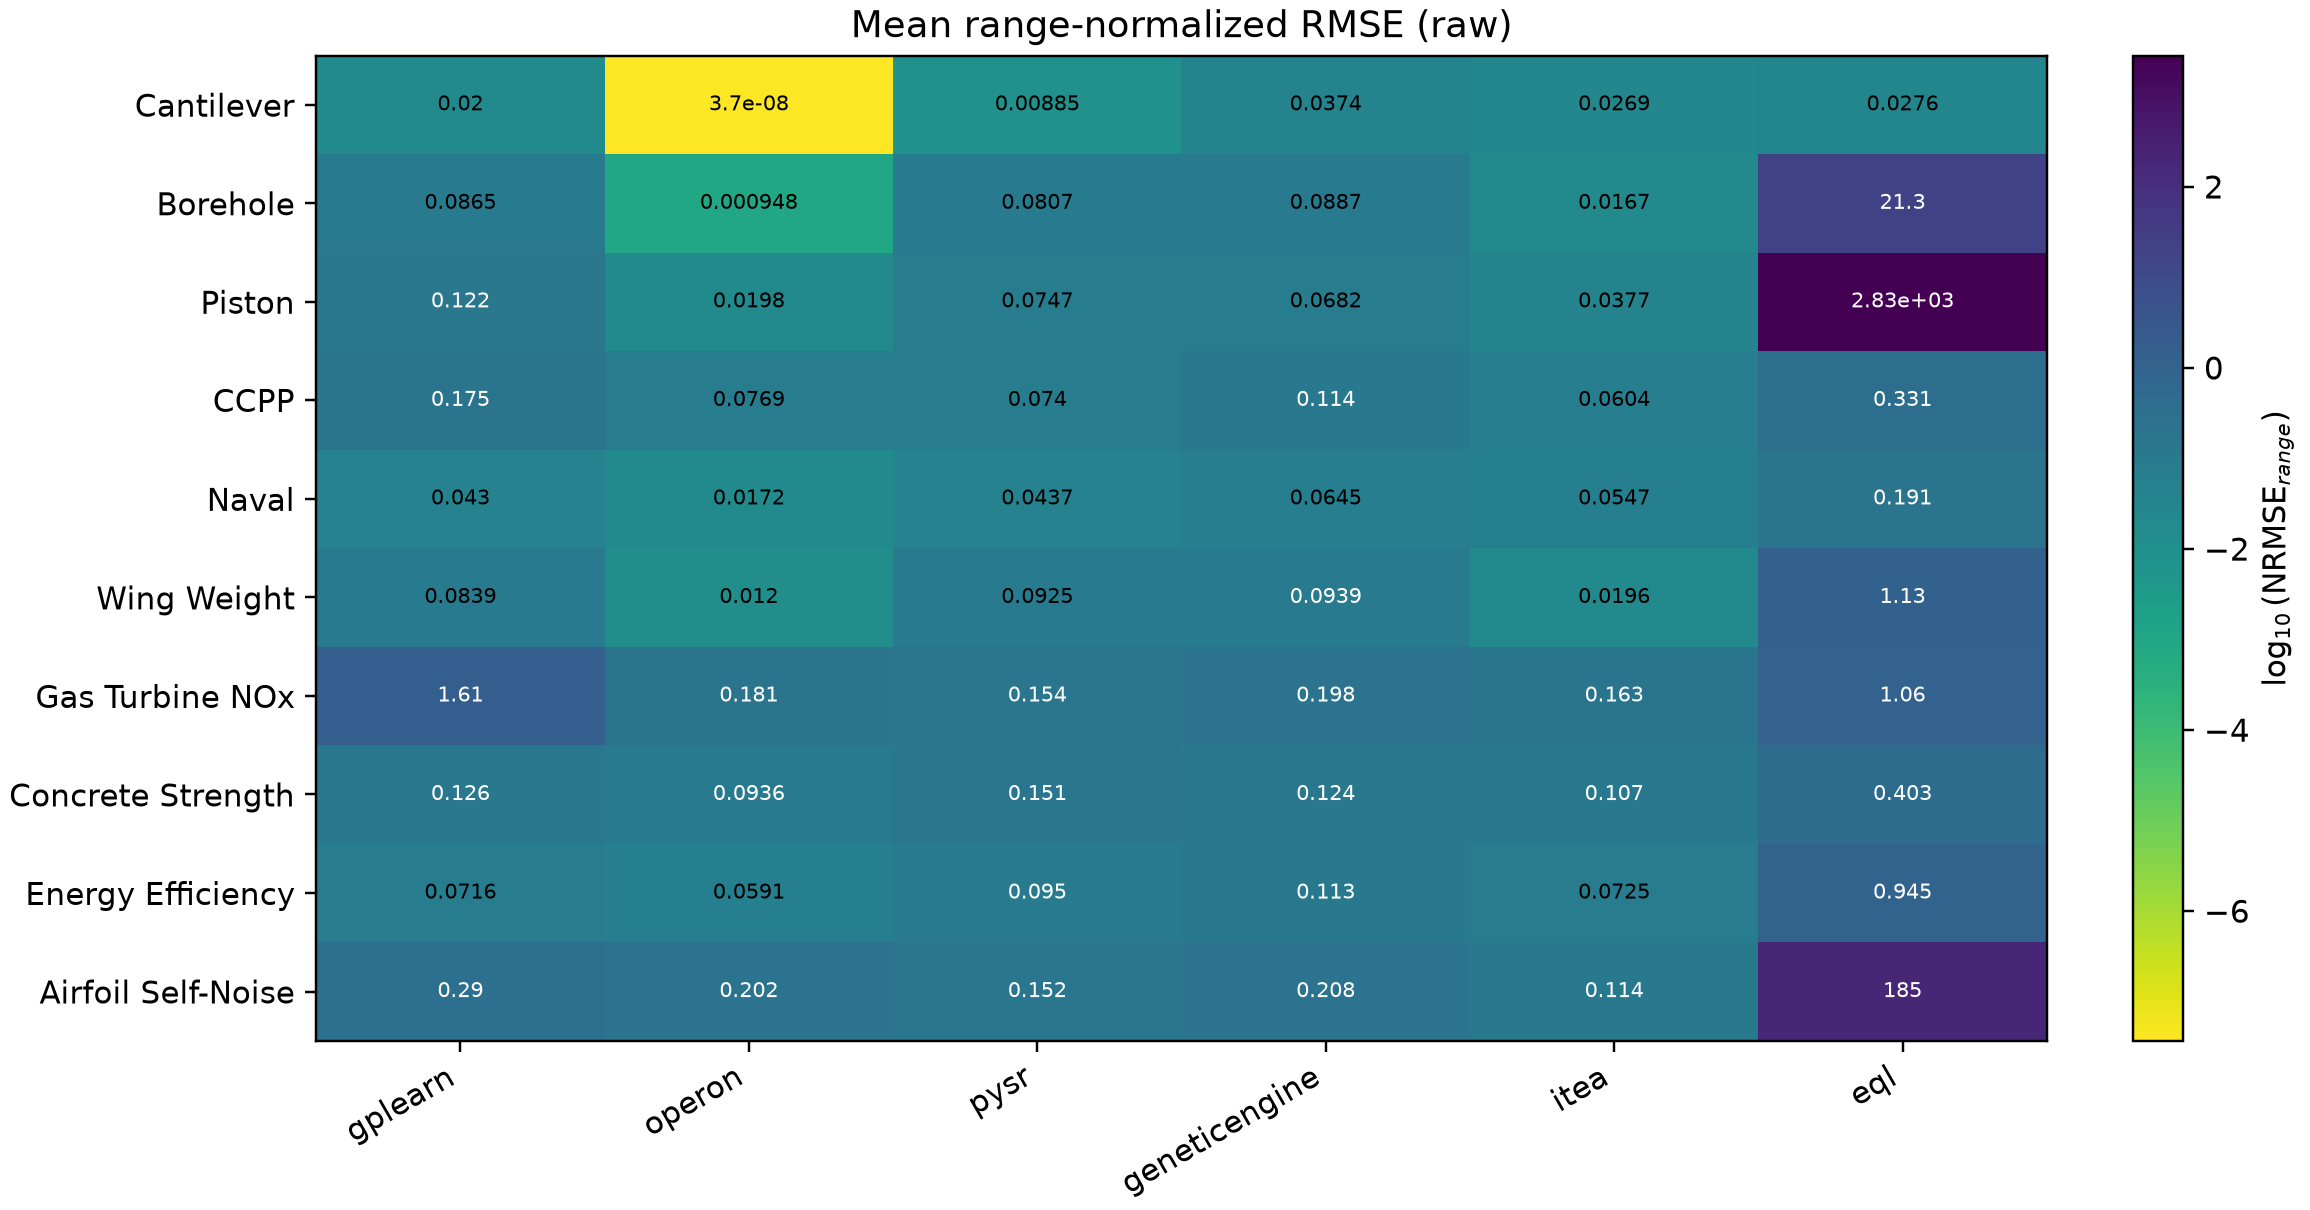
\includegraphics[width=0.96\textwidth]{images/results/nrmse_heatmap_raw.png}
    \caption{Mean range-normalized RMSE by framework and problem using raw inputs. Cell colors represent the base-10 logarithm of NRMSE, while annotations show the untransformed values.}
    \label{fig:results-nrmse-raw}
\end{figure}

\begin{figure}[H]
    \centering
    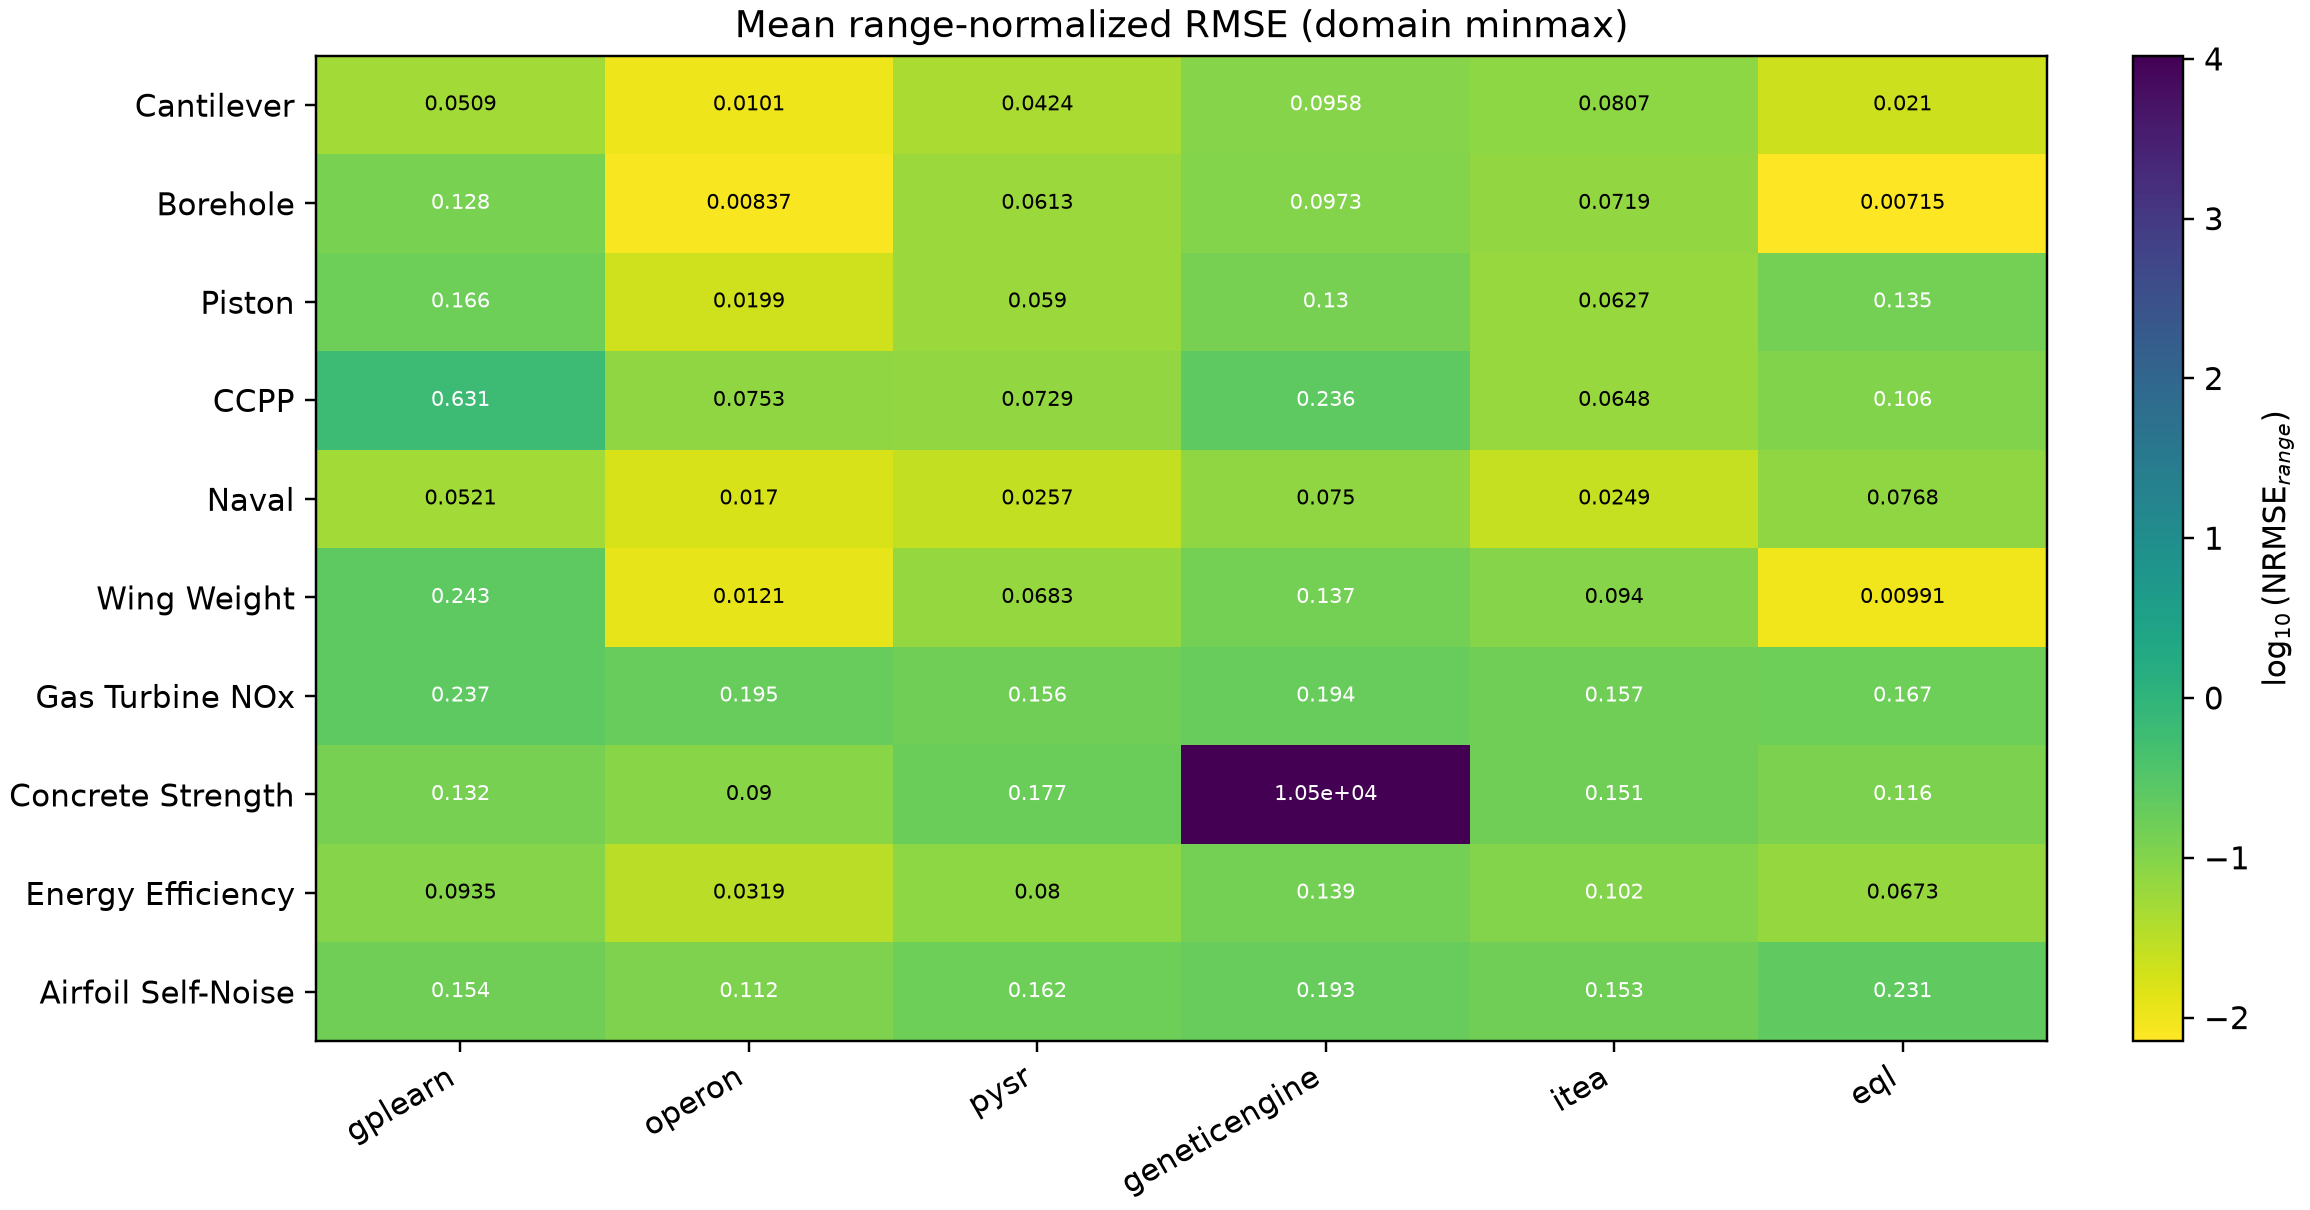
\includegraphics[width=0.96\textwidth]{images/results/nrmse_heatmap_domain_minmax.png}
    \caption{Mean range-normalized RMSE by framework and problem using domain-normalized inputs. Cell colors represent the base-10 logarithm of NRMSE, while annotations show the untransformed values.}
    \label{fig:results-nrmse-domain}
\end{figure}

\begin{figure}[H]
    \centering
    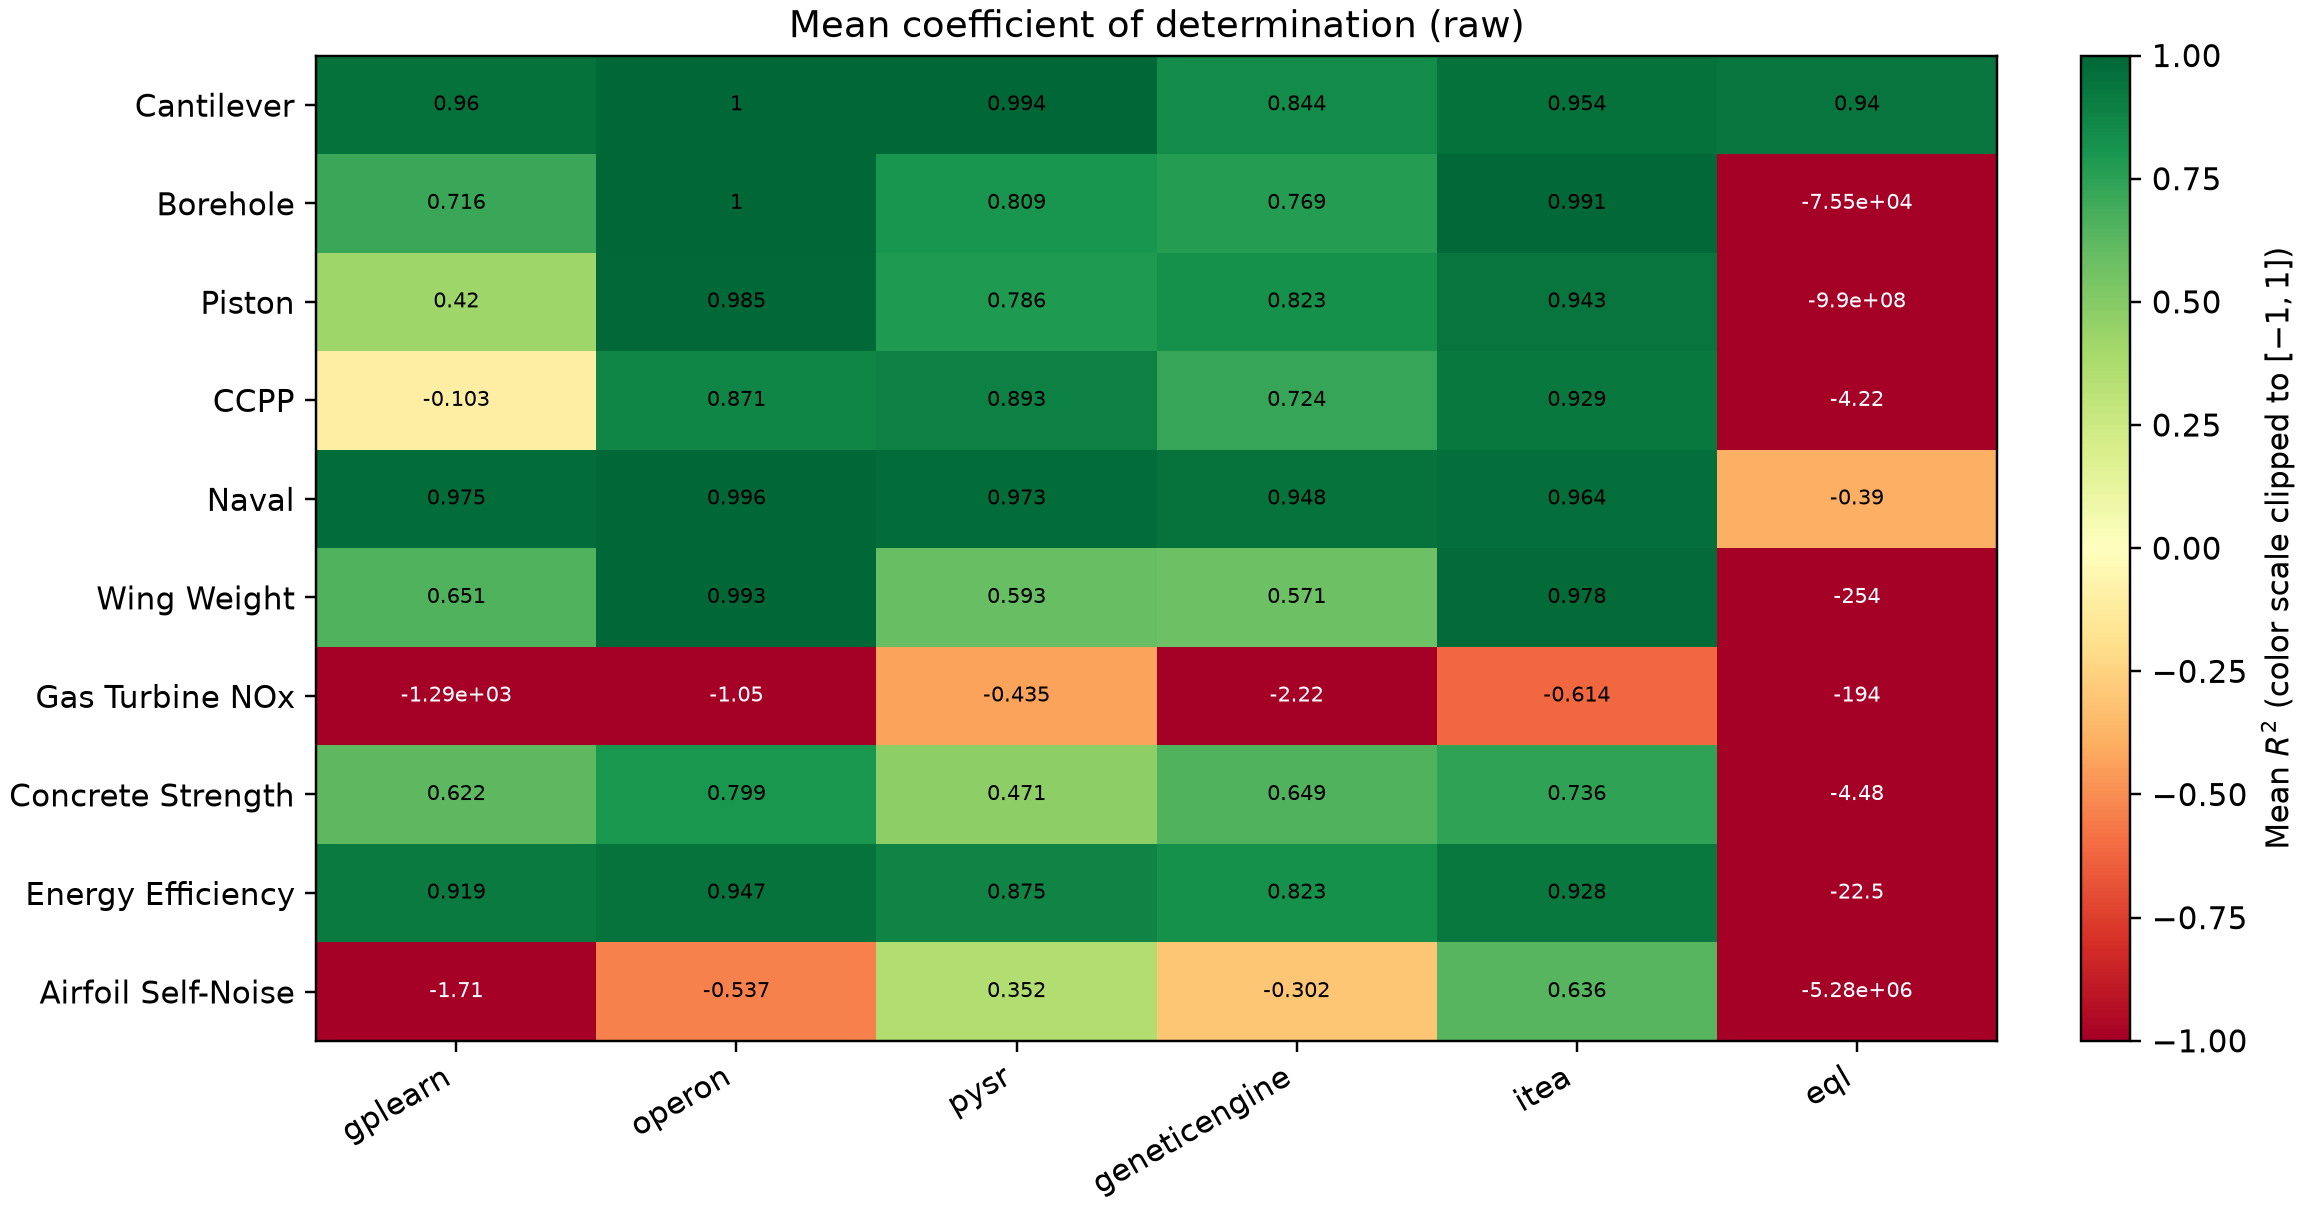
\includegraphics[width=0.96\textwidth]{images/results/r2_heatmap_raw.png}
    \caption{Mean coefficient of determination by framework and problem using raw inputs. The color scale is clipped to $[-1,1]$, while annotations report the untruncated values.}
    \label{fig:results-r2-raw}
\end{figure}

\begin{figure}[H]
    \centering
    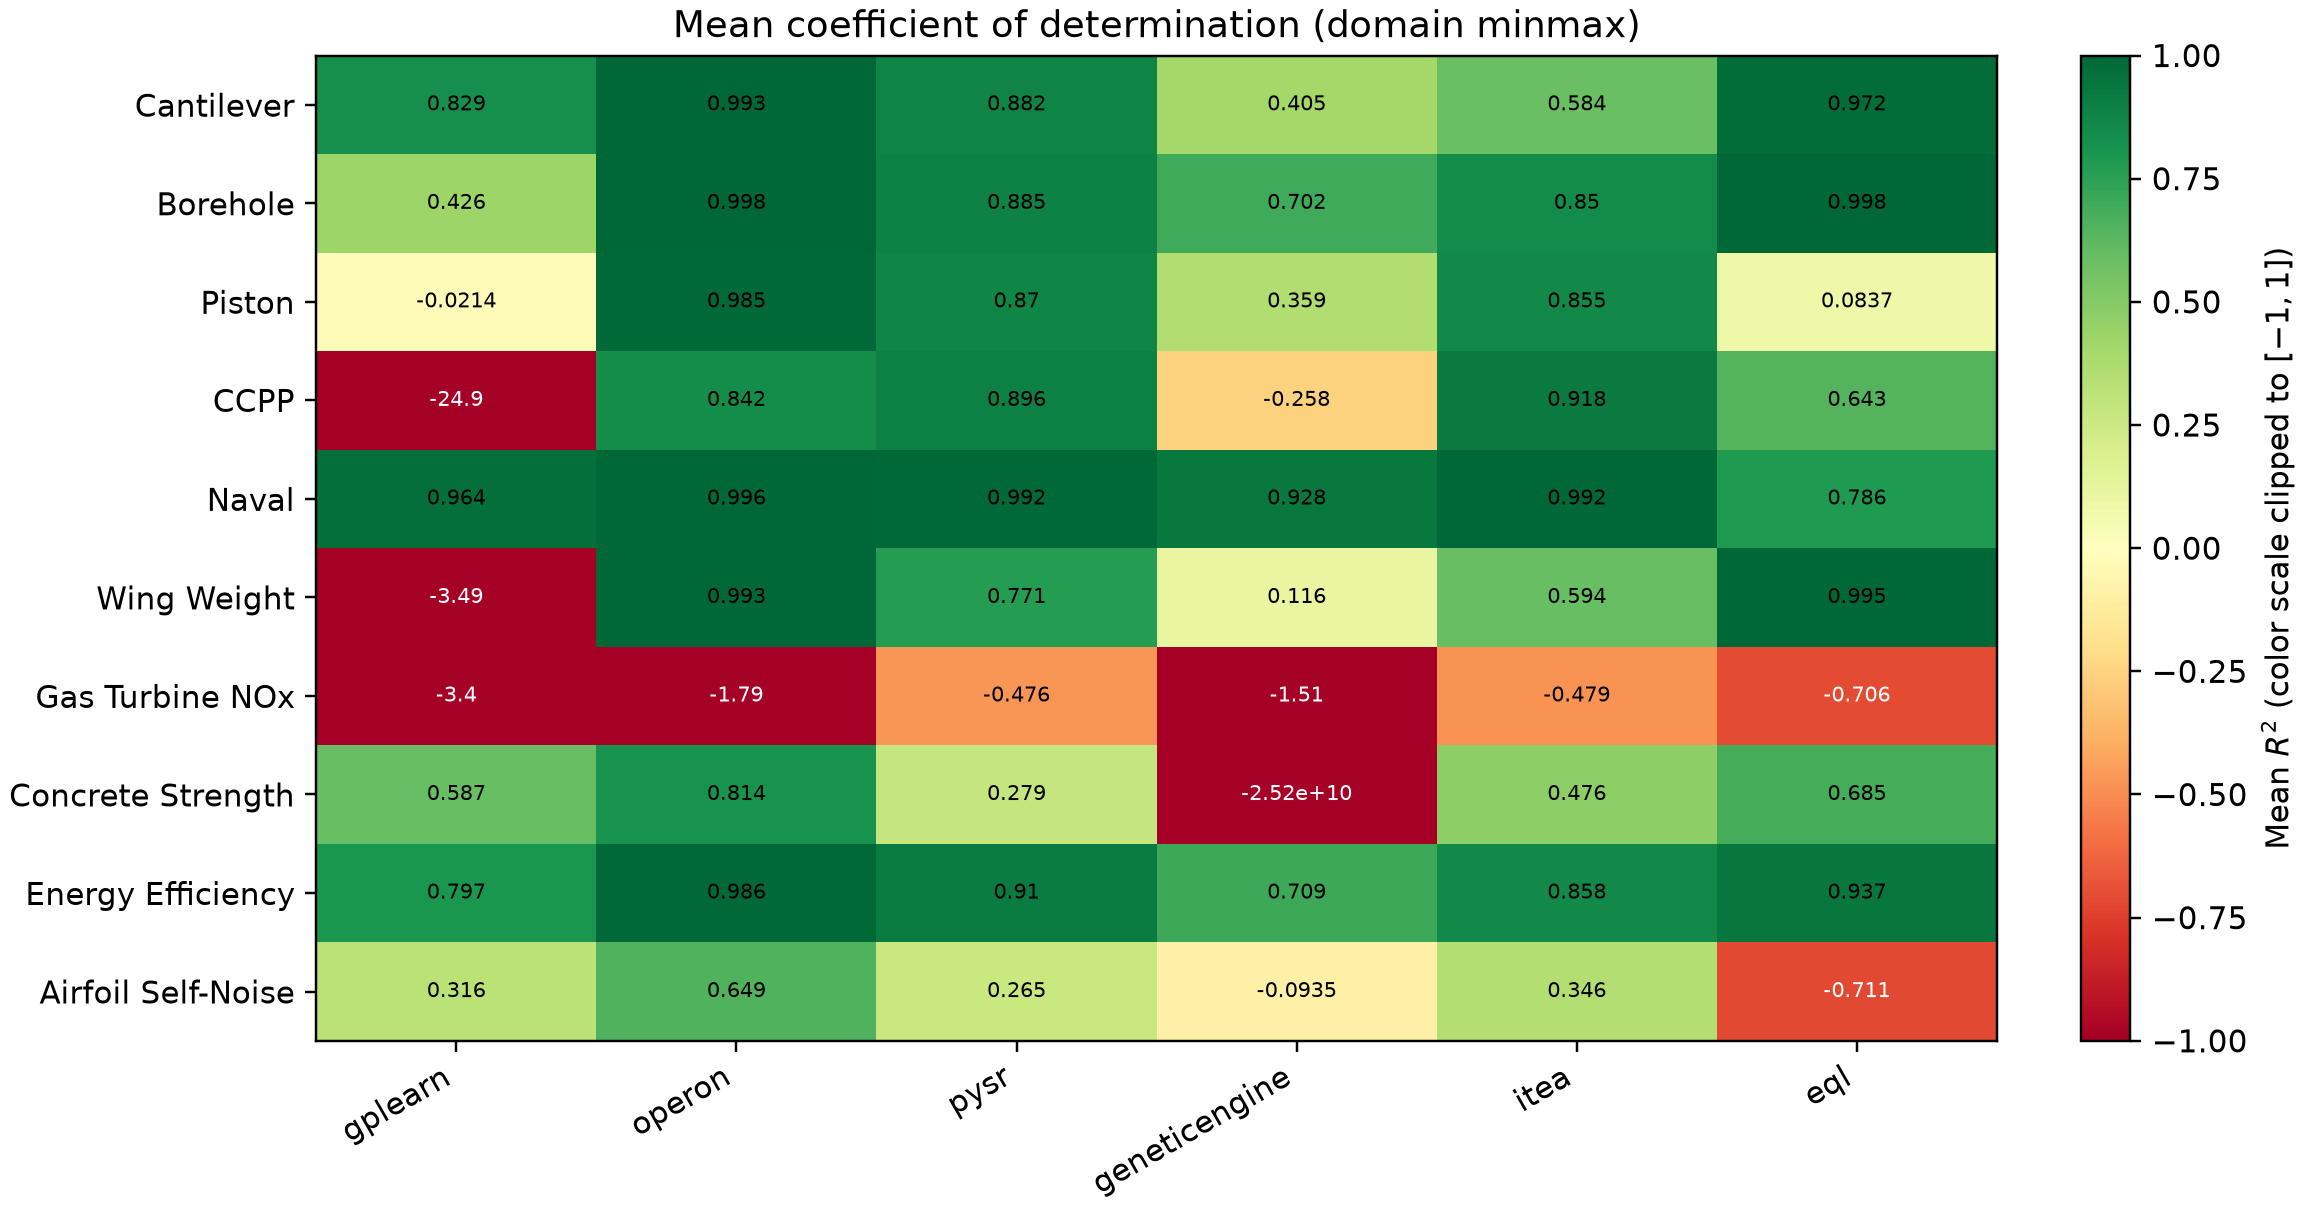
\includegraphics[width=0.96\textwidth]{images/results/r2_heatmap_domain_minmax.png}
    \caption{Mean coefficient of determination by framework and problem using domain-normalized inputs. The color scale is clipped to $[-1,1]$, while annotations report the untruncated values.}
    \label{fig:results-r2-domain}
\end{figure}

Across the 20 problem--scaling combinations, Operon achieved the lowest mean NRMSE in 13 cases. ITEA was best in three cases, while PySR and EQL were each best in two. Neither gplearn nor GeneticEngine obtained the lowest mean NRMSE in any combination. When the 20 problem-level means are summarized by their median, Operon obtained the lowest NRMSE at 0.0259 and the highest median $R^2$ at 0.9849. ITEA and PySR formed the next group, with median NRMSE values of 0.0722 and 0.0773, respectively.

\begin{table}[H]
    \centering
    \caption{Overall predictive summary across the 20 problem--scaling combinations. Medians are calculated from problem-level means, and wins count the lowest mean NRMSE in each combination.}
    \label{tab:results-overall-predictive}
    \begin{tabular}{lrrr}
        \toprule
        Framework & Median NRMSE & Median $R^2$ & NRMSE wins \\
        \midrule
        gplearn & 0.1267 & 0.5064 & 0 \\
        Operon & 0.0259 & 0.9849 & 13 \\
        PySR & 0.0773 & 0.8396 & 2 \\
        GeneticEngine & 0.1187 & 0.6101 & 0 \\
        ITEA & 0.0722 & 0.8564 & 3 \\
        EQL & 0.1791 & -0.5483 & 2 \\
        \bottomrule
    \end{tabular}
\end{table}

\subsection{Performance by Problem}

Table~\ref{tab:results-problem-winners} reports the strongest framework for each problem and scaling condition. Operon led both conditions on Cantilever, Piston, Naval Propulsion, and Concrete Strength. It also led raw Borehole and both the normalized Energy Efficiency and Airfoil Self-Noise configurations. EQL produced the lowest mean NRMSE for normalized Borehole and Wing Weight, whereas ITEA led both CCPP conditions and raw Airfoil Self-Noise. PySR obtained the best result on Gas Turbine NOx under both scaling conditions.

\begin{longtable}{llrr}
\caption{Lowest mean NRMSE for each problem and input-scaling condition.}\label{tab:results-problem-winners}\\
\toprule
Problem & Scaling & Framework & Mean NRMSE \\
\midrule
\endfirsthead
\toprule
Problem & Scaling & Framework & Mean NRMSE \\
\midrule
\endhead
Cantilever & Raw & Operon & $3.70\times10^{-8}$ \\
Cantilever & Domain-normalized & Operon & 0.0101 \\
Borehole & Raw & Operon & 0.0009 \\
Borehole & Domain-normalized & EQL & 0.0072 \\
Piston & Raw & Operon & 0.0198 \\
Piston & Domain-normalized & Operon & 0.0199 \\
CCPP & Raw & ITEA & 0.0604 \\
CCPP & Domain-normalized & ITEA & 0.0648 \\
Naval Propulsion & Raw & Operon & 0.0172 \\
Naval Propulsion & Domain-normalized & Operon & 0.0170 \\
Wing Weight & Raw & Operon & 0.0120 \\
Wing Weight & Domain-normalized & EQL & 0.0099 \\
Gas Turbine NOx & Raw & PySR & 0.1536 \\
Gas Turbine NOx & Domain-normalized & PySR & 0.1563 \\
Concrete Strength & Raw & Operon & 0.0936 \\
Concrete Strength & Domain-normalized & Operon & 0.0900 \\
Energy Efficiency & Raw & Operon & 0.0591 \\
Energy Efficiency & Domain-normalized & Operon & 0.0319 \\
Airfoil Self-Noise & Raw & ITEA & 0.1142 \\
Airfoil Self-Noise & Domain-normalized & Operon & 0.1120 \\
\bottomrule
\end{longtable}

The analytical problems generally admitted substantially lower errors than the external datasets, although performance differed between methods. Operon nearly recovered the Cantilever mapping numerically under raw inputs and reached mean NRMSE below 0.02 on several analytical configurations. The Gas Turbine NOx problem was the most consistently difficult empirical task, even its best framework produced negative mean $R^2$ in both conditions ($-0.4349$ for raw inputs and $-0.4763$ for normalized inputs). Airfoil Self-Noise and Concrete Strength were also more difficult than the strongest analytical results, but their best mean $R^2$ values remained positive at approximately 0.65 and 0.81, respectively.

\subsection{Analytical and Empirical Problems}

The four analytical problems and six external datasets serve different evaluation roles. Table~\ref{tab:results-problem-types} summarizes their mean-NRMSE distributions across frameworks. The median result on analytical problems was lower under raw inputs than under normalized inputs, whereas the median over external problems was almost unchanged. The analytical median nevertheless conceals several poor individual results, particularly the extreme raw-input EQL errors on Piston and Wing Weight. Conversely, the external group contains both the comparatively well-predicted Energy Efficiency task and the substantially harder Gas Turbine NOx task.

\begin{table}[H]
    \centering
    \caption{Median of the framework-level mean NRMSE values by problem type and scaling condition.}
    \label{tab:results-problem-types}
    \begin{tabular}{lrr}
        \toprule
        Problem type & Raw inputs & Domain-normalized inputs \\
        \midrule
        Analytical problems & 0.0546 & 0.0655 \\
        External datasets & 0.1247 & 0.1240 \\
        \bottomrule
    \end{tabular}
\end{table}

\section{Effects of Input Scaling and Repetition Variability}

In addition to average predictive performance, the benchmark evaluates whether the results change when the inputs are domain-normalized and how strongly they vary across repeated trials. This analysis reveals whether a framework's observed performance is consistent across preprocessing conditions and repetitions.

\subsection{Effect of Domain Normalization}

The effect of domain normalization was framework-dependent rather than uniformly beneficial. Table~\ref{tab:results-scaling-effect} compares each framework's normalized-input mean NRMSE with its raw-input result on the same problem. EQL improved on all ten problems and showed the largest median reduction, with a normalized-to-raw NRMSE ratio of 0.114. PySR improved on six problems and Operon on five, while Operon's median ratio remained close to one. gplearn, GeneticEngine, and ITEA each improved on two problems, and their median ratios were above one.

\begin{table}[H]
    \centering
    \caption{Effect of domain normalization. The ratio is calculated per problem from the normalized and raw mean NRMSE and then summarized by its median; values below one favor normalization.}
    \label{tab:results-scaling-effect}
    \begin{tabular}{lrr}
        \toprule
        Framework & Problems improved (of 10) & Median NRMSE ratio \\
        \midrule
        gplearn & 2 & 1.336 \\
        Operon & 5 & 0.998 \\
        PySR & 6 & 0.914 \\
        GeneticEngine & 2 & 1.344 \\
        ITEA & 2 & 1.406 \\
        EQL & 10 & 0.114 \\
        \bottomrule
    \end{tabular}
\end{table}

Figure~\ref{fig:results-scaling-effect} displays the paired raw and normalized results for each framework and problem. Points below the diagonal indicate an improvement after normalization. The figure highlights that EQL's aggregate improvement was driven in part by avoiding very large raw-input errors, whereas the other frameworks showed smaller and less consistent shifts in either direction.

\begin{figure}[H]
    \centering
    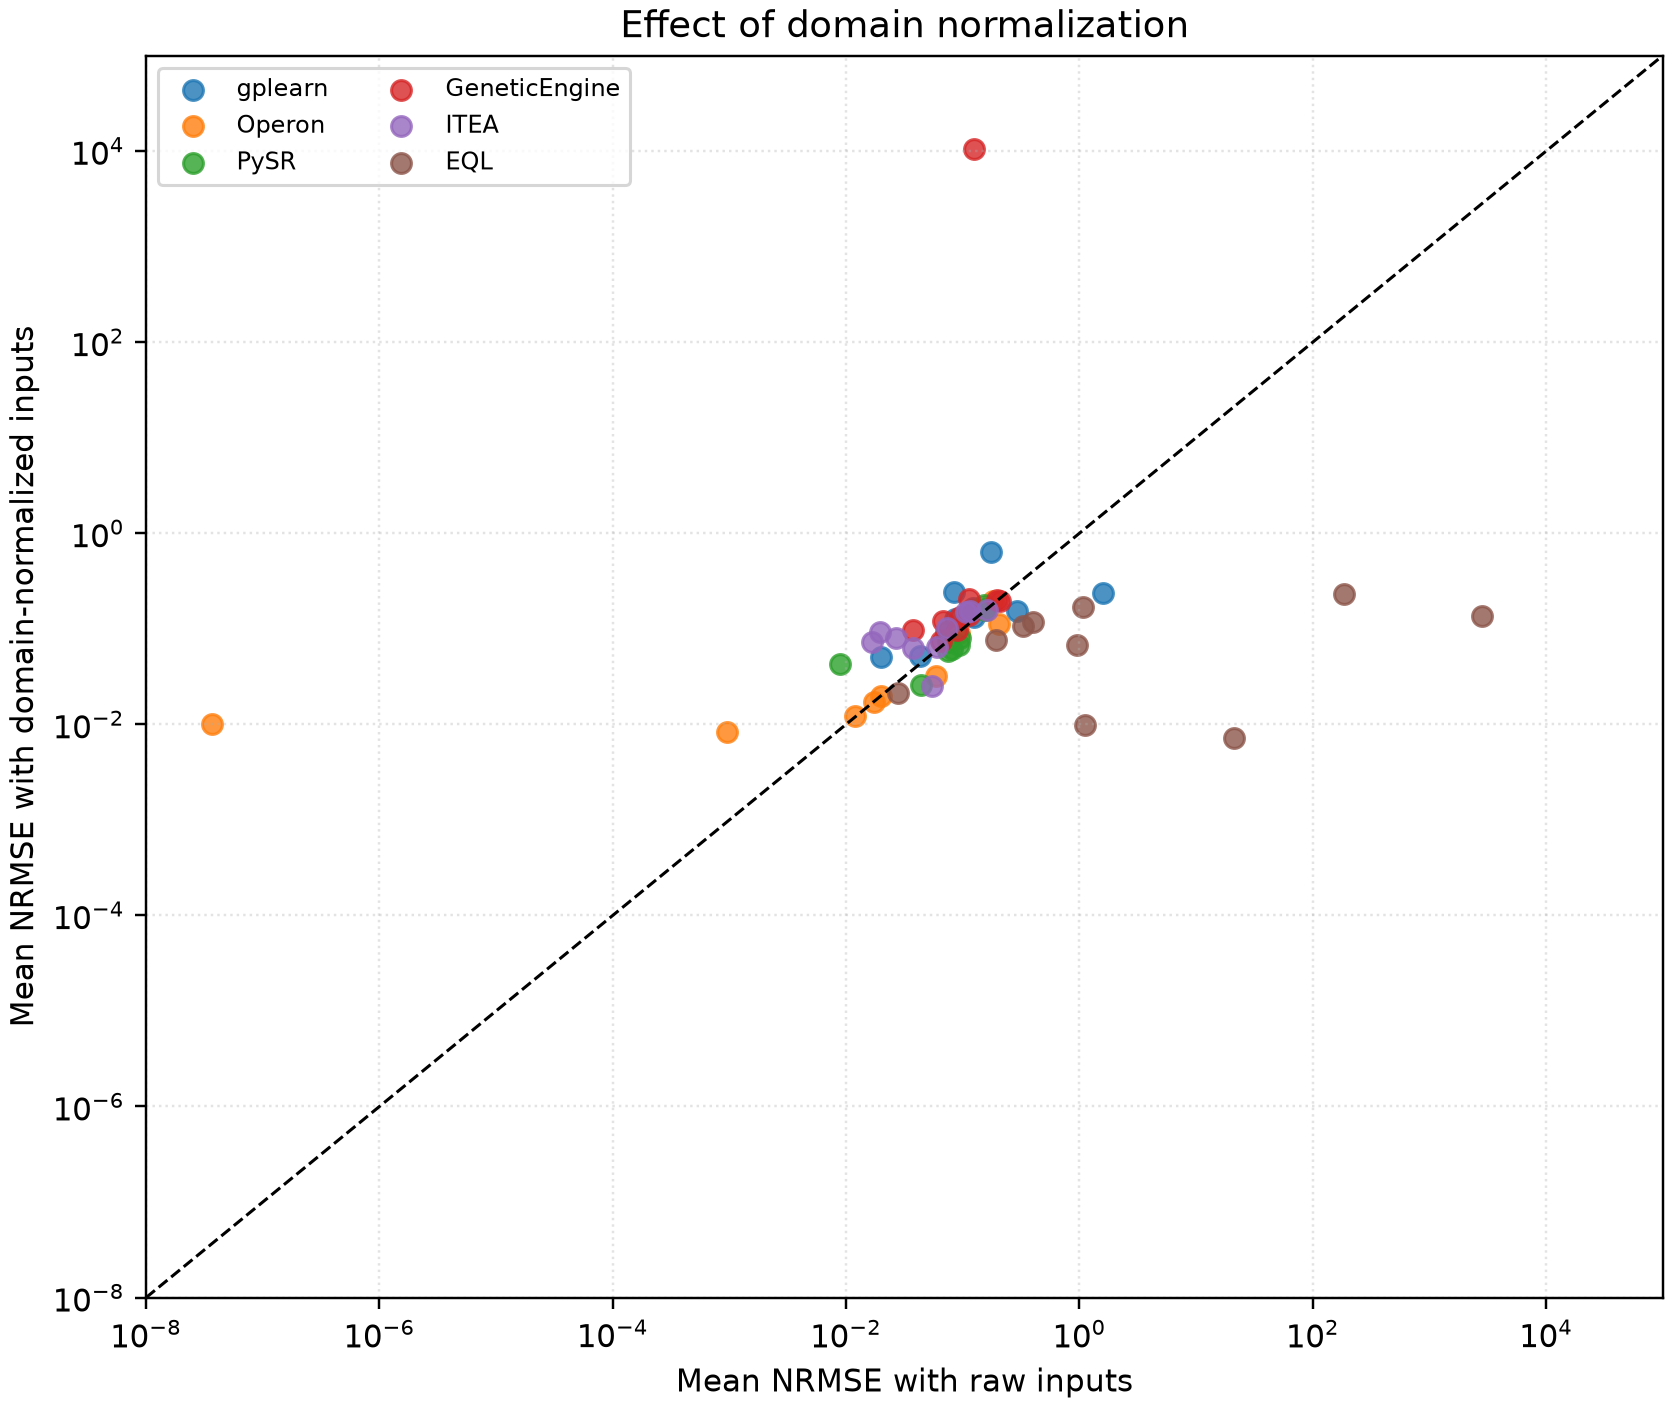
\includegraphics[width=0.88\textwidth]{images/results/normalization_effect.png}
    \caption{Effect of domain normalization on mean range-normalized RMSE. The diagonal represents equal error under both input-scaling conditions.}
    \label{fig:results-scaling-effect}
\end{figure}

\subsection{Stability Across Repetitions}

Repetition variability was evaluated using the sample standard deviation of NRMSE within each framework--problem--scaling configuration. Table~\ref{tab:results-repetition-stability} summarizes these values by taking their median across problems. Operon and PySR showed comparatively small dispersion under both scaling conditions. gplearn and GeneticEngine were more variable, particularly with normalized inputs. EQL was highly unstable with raw inputs because individual repetitions produced very large prediction errors, while normalization reduced its median standard deviation substantially.

\begin{table}[H]
    \centering
    \caption{Median problem-level sample standard deviation of NRMSE across repetitions.}
    \label{tab:results-repetition-stability}
    \begin{tabular}{lrr}
        \toprule
        Framework & Raw inputs & Domain-normalized inputs \\
        \midrule
        gplearn & 0.0306 & 0.0469 \\
        Operon & 0.0038 & 0.0034 \\
        PySR & 0.0121 & 0.0084 \\
        GeneticEngine & 0.0185 & 0.0372 \\
        ITEA & 0.0002 & $<0.0001$ \\
        EQL & 1.2407 & 0.0192 \\
        \bottomrule
    \end{tabular}
\end{table}

ITEA produced nearly identical results across repetitions. This observation should not be interpreted as evidence that a controllable random seed made the method reproducible, because the evaluated adapter does not expose a supported repetition-seed parameter. Instead, it indicates that the evaluated configuration returned almost unchanged results when invoked repeatedly on the same fixed tables. Figures~\ref{fig:results-repetition-raw} and~\ref{fig:results-repetition-domain} show the full distributions of repetition-level NRMSE values and make both narrow distributions and isolated failures or extreme errors visible. Separate vertical ranges are used so that the substantially narrower normalized-input distribution remains legible.

\begin{figure}[H]
    \centering
    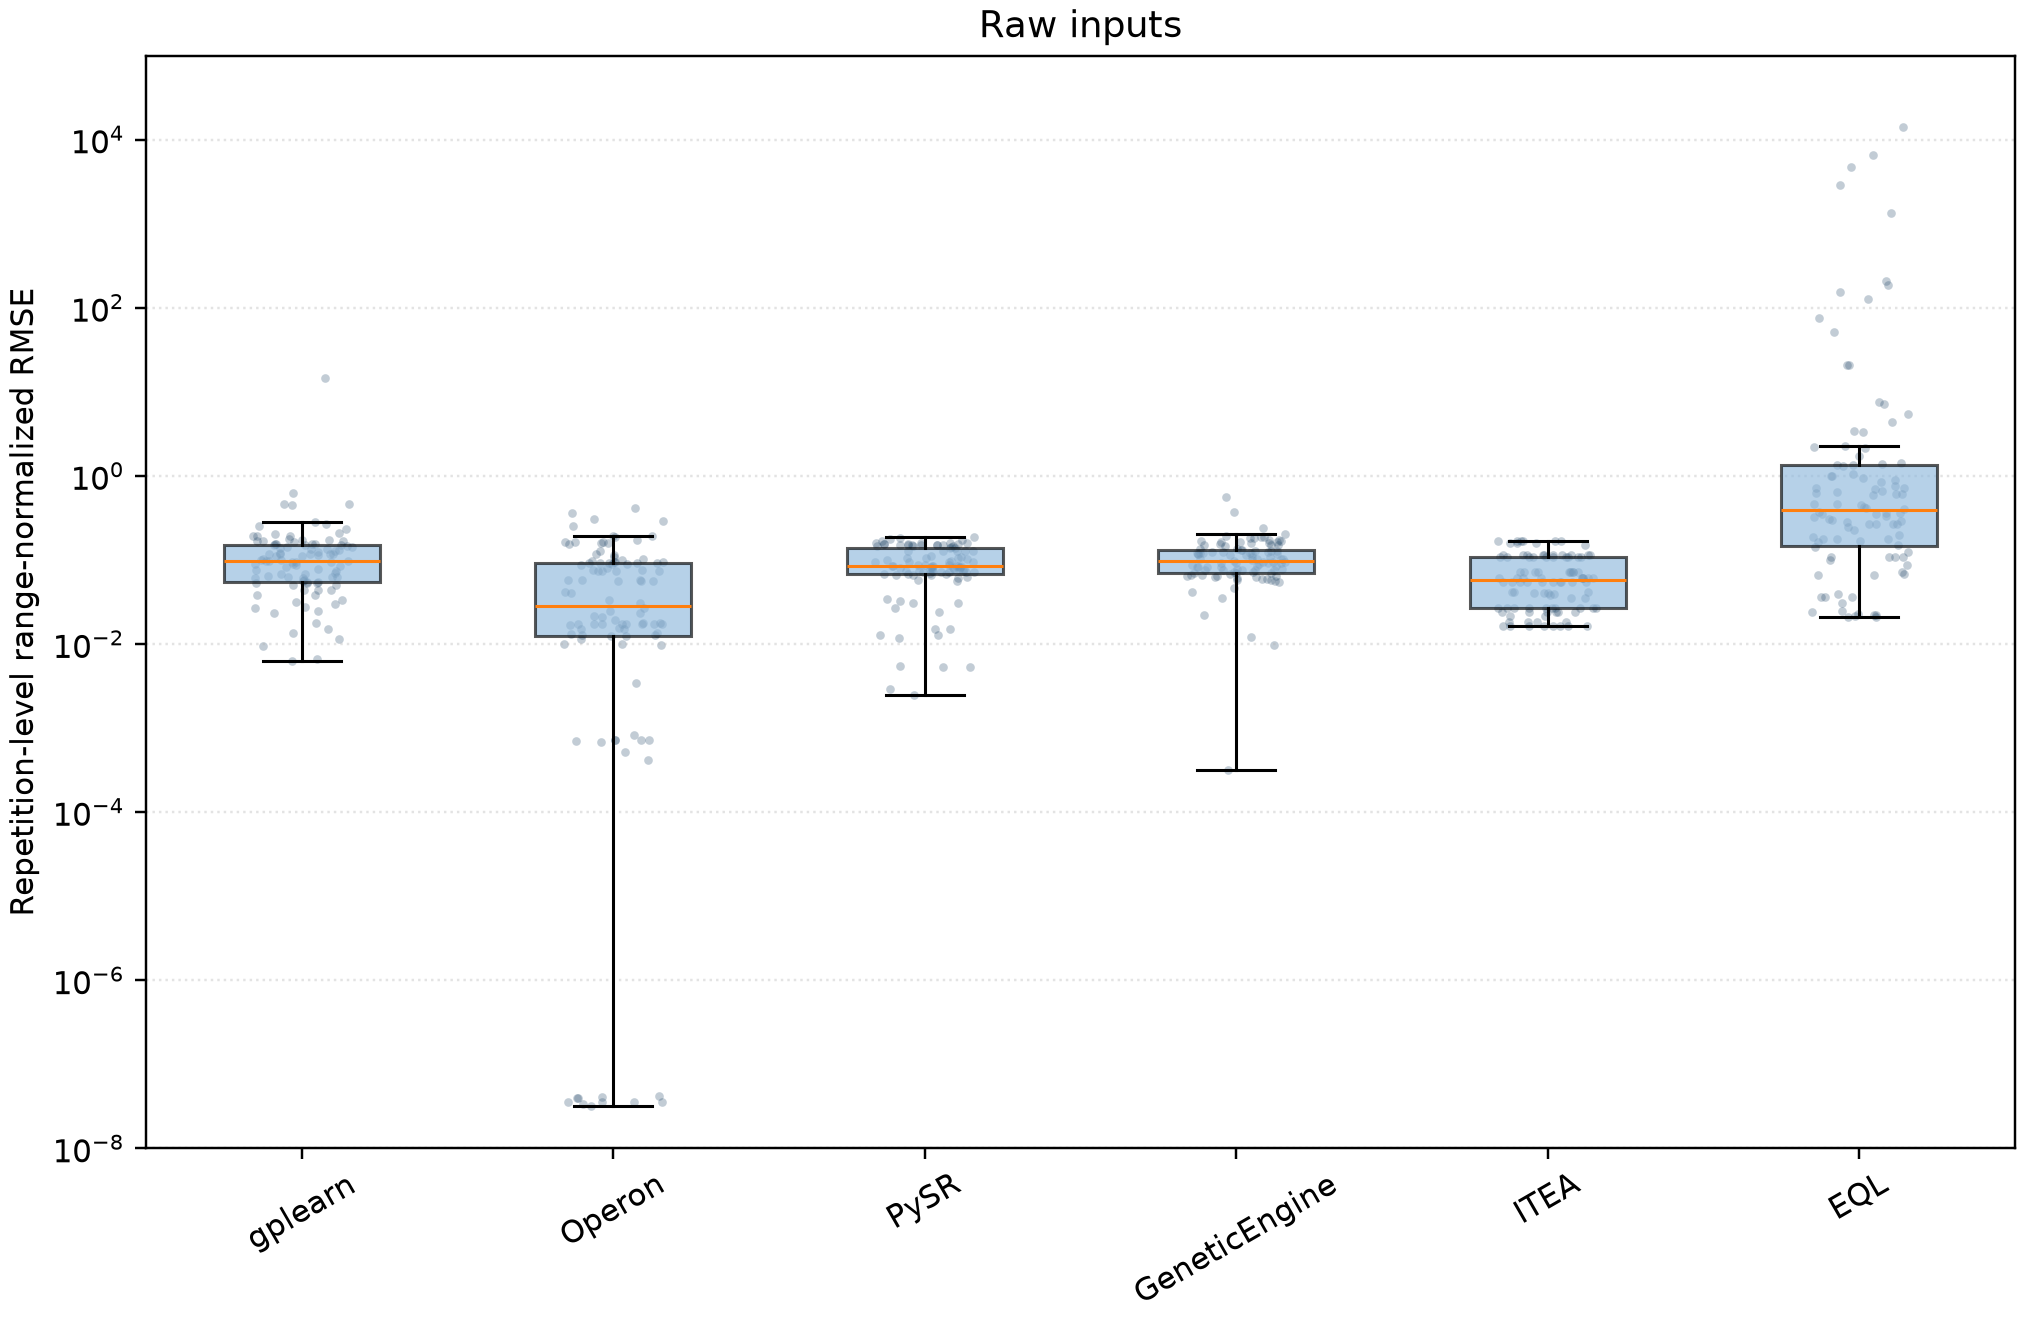
\includegraphics[width=0.95\textwidth]{images/results/repetition_nrmse_raw.png}
    \caption{Distribution of repetition-level range-normalized RMSE by framework using raw inputs. Points represent successful trials across all problems and boxes summarize their distributions.}
    \label{fig:results-repetition-raw}
\end{figure}

\begin{figure}[H]
    \centering
    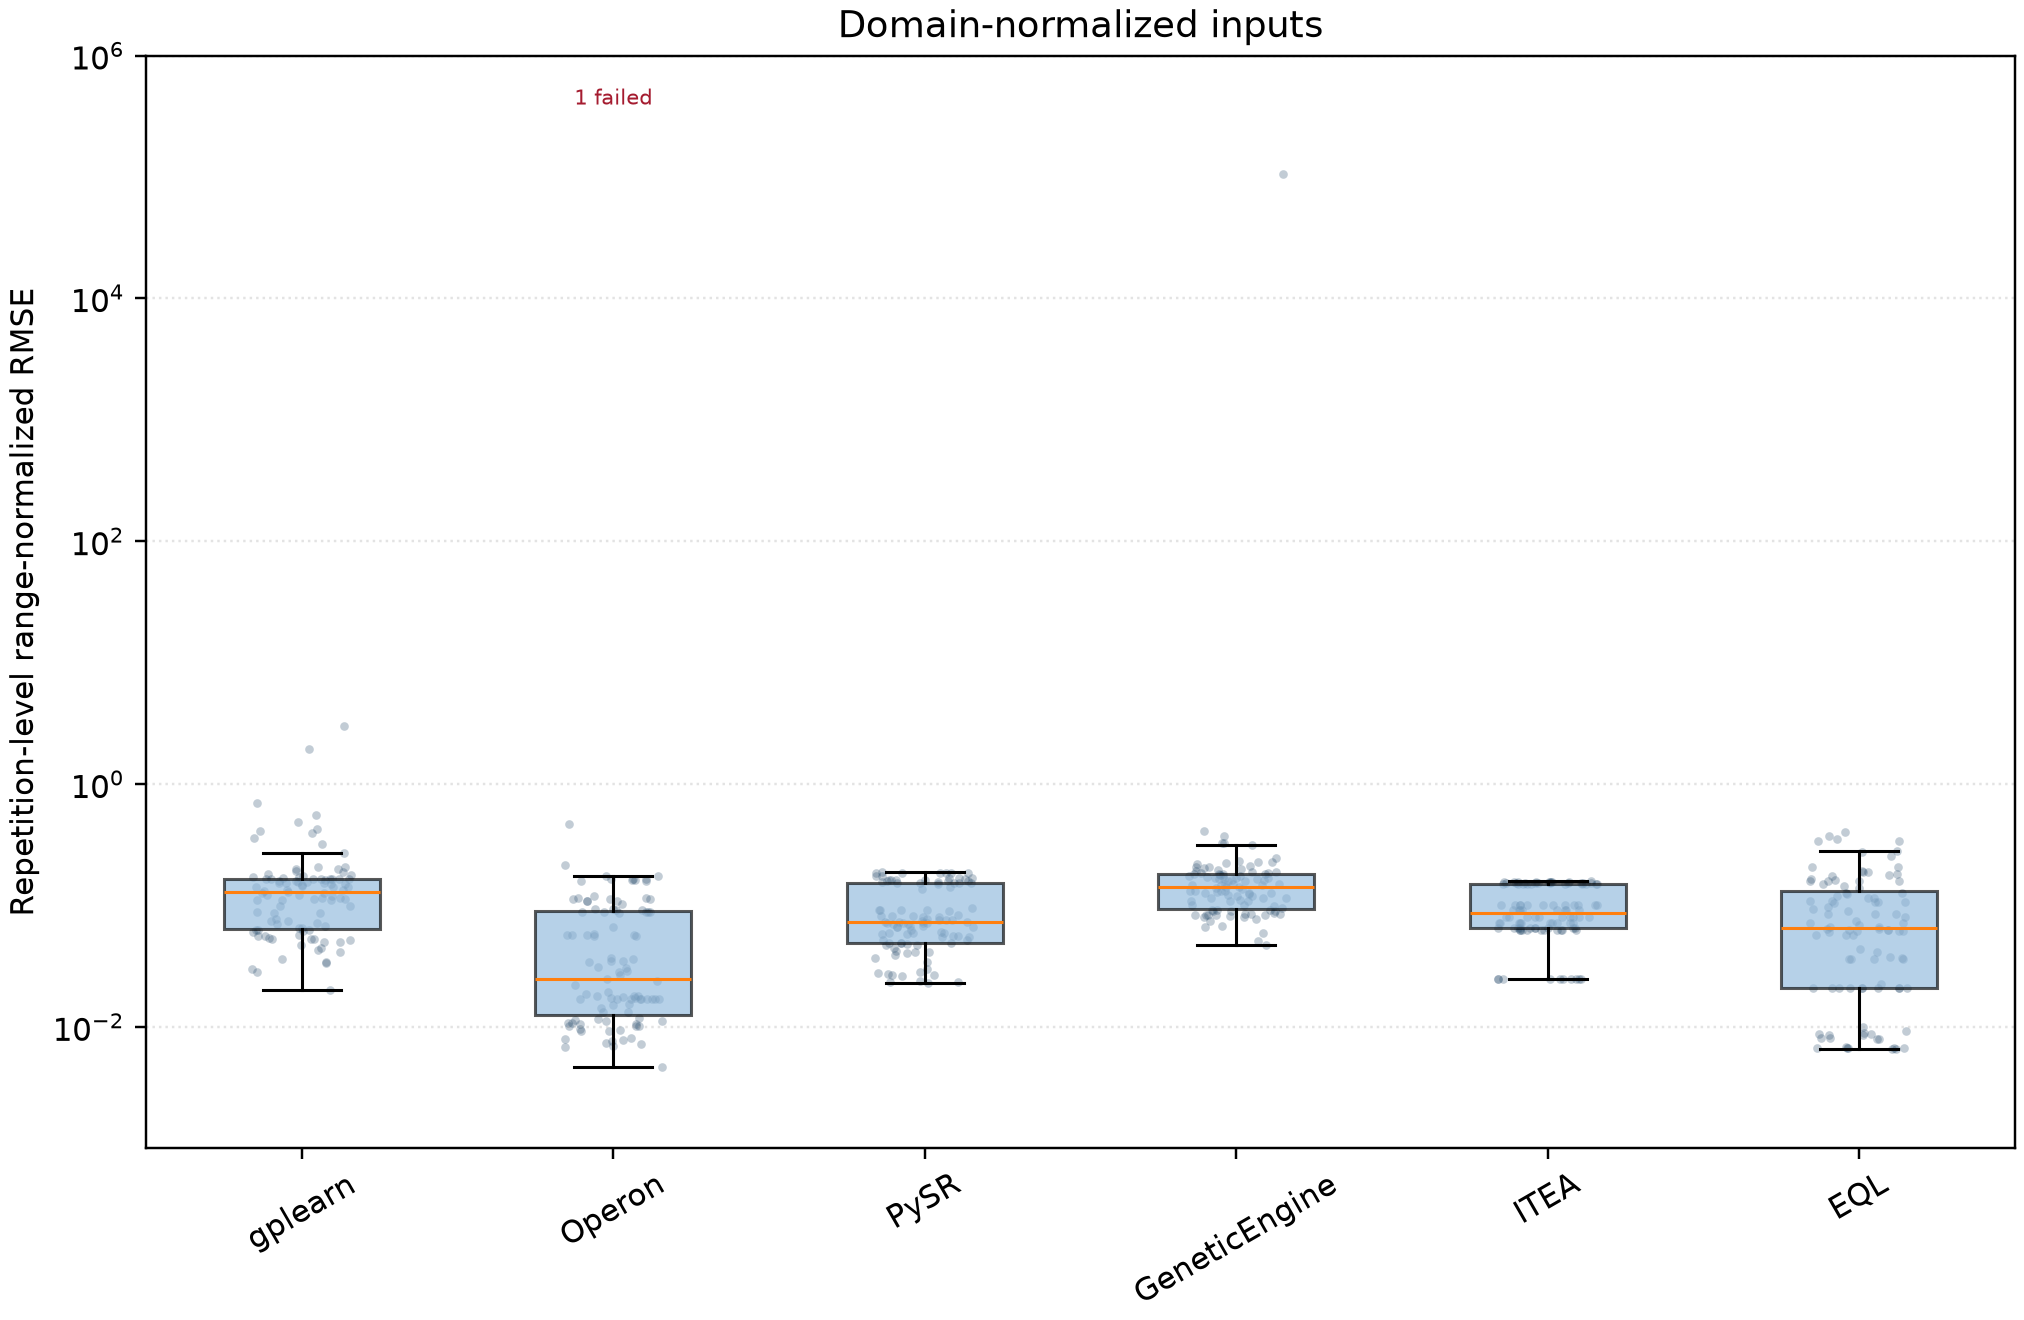
\includegraphics[width=0.95\textwidth]{images/results/repetition_nrmse_domain_minmax.png}
    \caption{Distribution of repetition-level range-normalized RMSE by framework using domain-normalized inputs. Points represent successful trials across all problems, boxes summarize their distributions, and red annotations report failed trials.}
    \label{fig:results-repetition-domain}
\end{figure}

\section{Symbolic Model Properties}

The returned equations are compared not only through their predictions but also through properties of their symbolic representations. This section examines expression-tree complexity and reports how frequently the common symbolic simplification procedure completed or required a fallback to the unsimplified expression.

\subsection{Expression Complexity}

Expression complexity varied substantially between frameworks. Table~\ref{tab:results-complexity-summary} reports the median, across the 20 problem--scaling combinations, of each combination's mean simplified node count. On this measure, PySR returned the smallest parsed expressions, followed by ITEA and GeneticEngine. Operon, despite leading predictive performance, returned larger expressions than these three frameworks. gplearn had the largest median node count. These comparisons describe syntactic expression size and do not by themselves measure semantic clarity or scientific usefulness.

\begin{table}[H]
    \centering
    \caption{Median of the problem-level mean simplified expression-tree node counts across both scaling conditions. Only trials for which simplification completed are included.}
    \label{tab:results-complexity-summary}
    \begin{tabular}{lr}
        \toprule
        Framework & Median simplified node count \\
        \midrule
        gplearn & 108.39 \\
        Operon & 66.00 \\
        PySR & 11.21 \\
        GeneticEngine & 26.10 \\
        ITEA & 21.60 \\
        EQL & 51.65 \\
        \bottomrule
    \end{tabular}
\end{table}

Figures~\ref{fig:results-complexity-raw} and~\ref{fig:results-complexity-domain} show that expression size is also dependent on the problem and scaling condition, so the aggregate ordering did not hold uniformly in every cell. Complexity must therefore be considered alongside prediction error at the framework--problem level rather than interpreted only through one framework-wide average.

\begin{figure}[H]
    \centering
    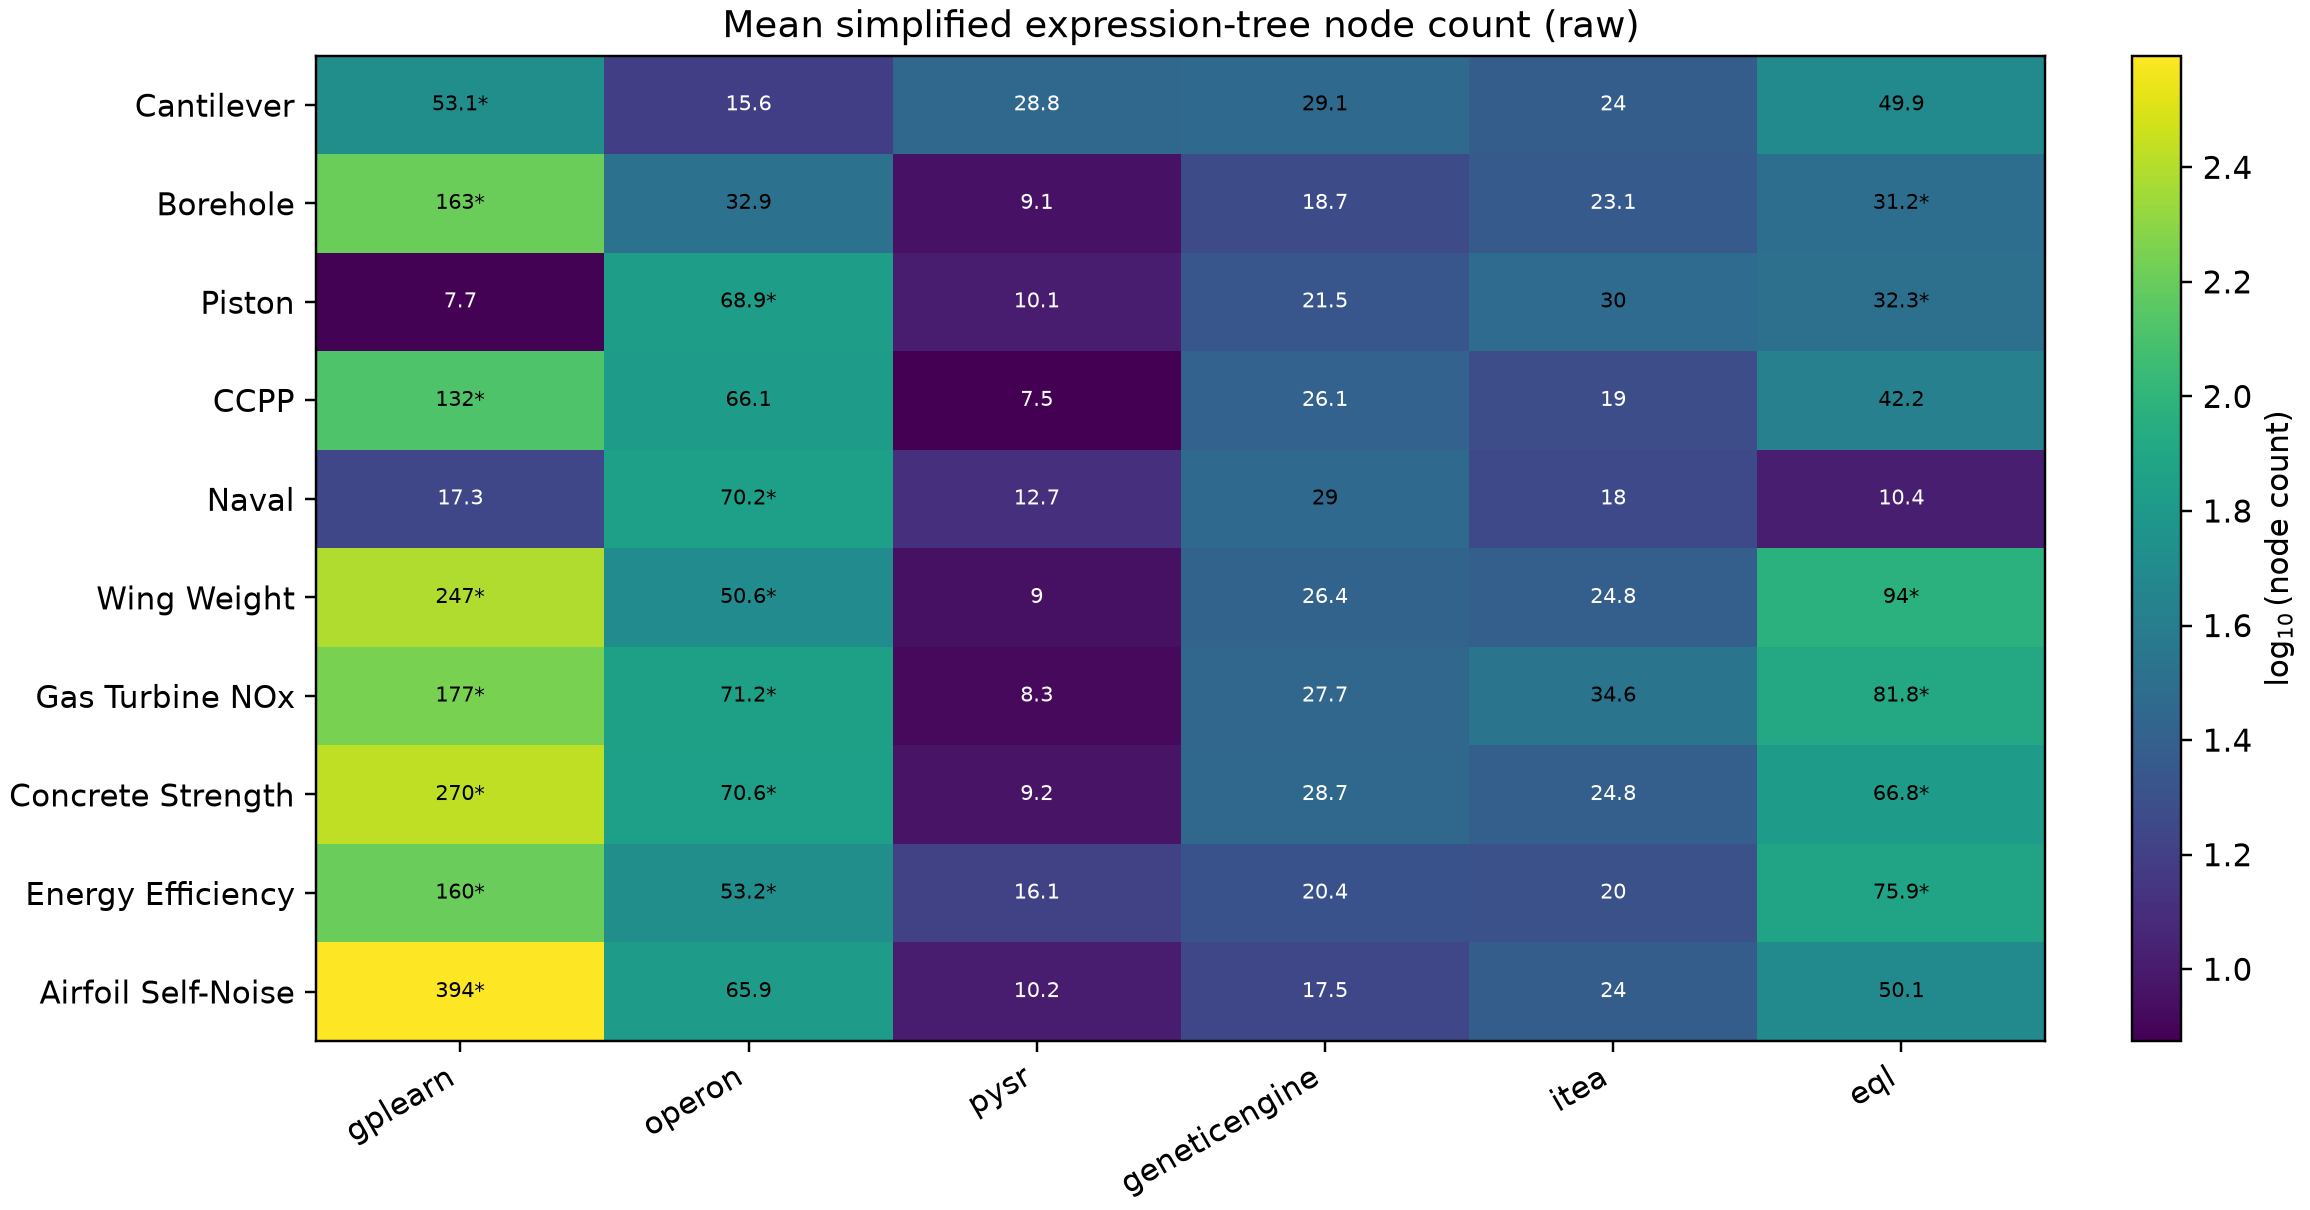
\includegraphics[width=0.96\textwidth]{images/results/complexity_heatmap_raw.png}
    \caption{Mean simplified expression-tree node count by framework and problem using raw inputs. An asterisk indicates that at least one expression in the cell required the unsimplified complexity fallback and was excluded from the displayed simplified mean.}
    \label{fig:results-complexity-raw}
\end{figure}

\begin{figure}[H]
    \centering
    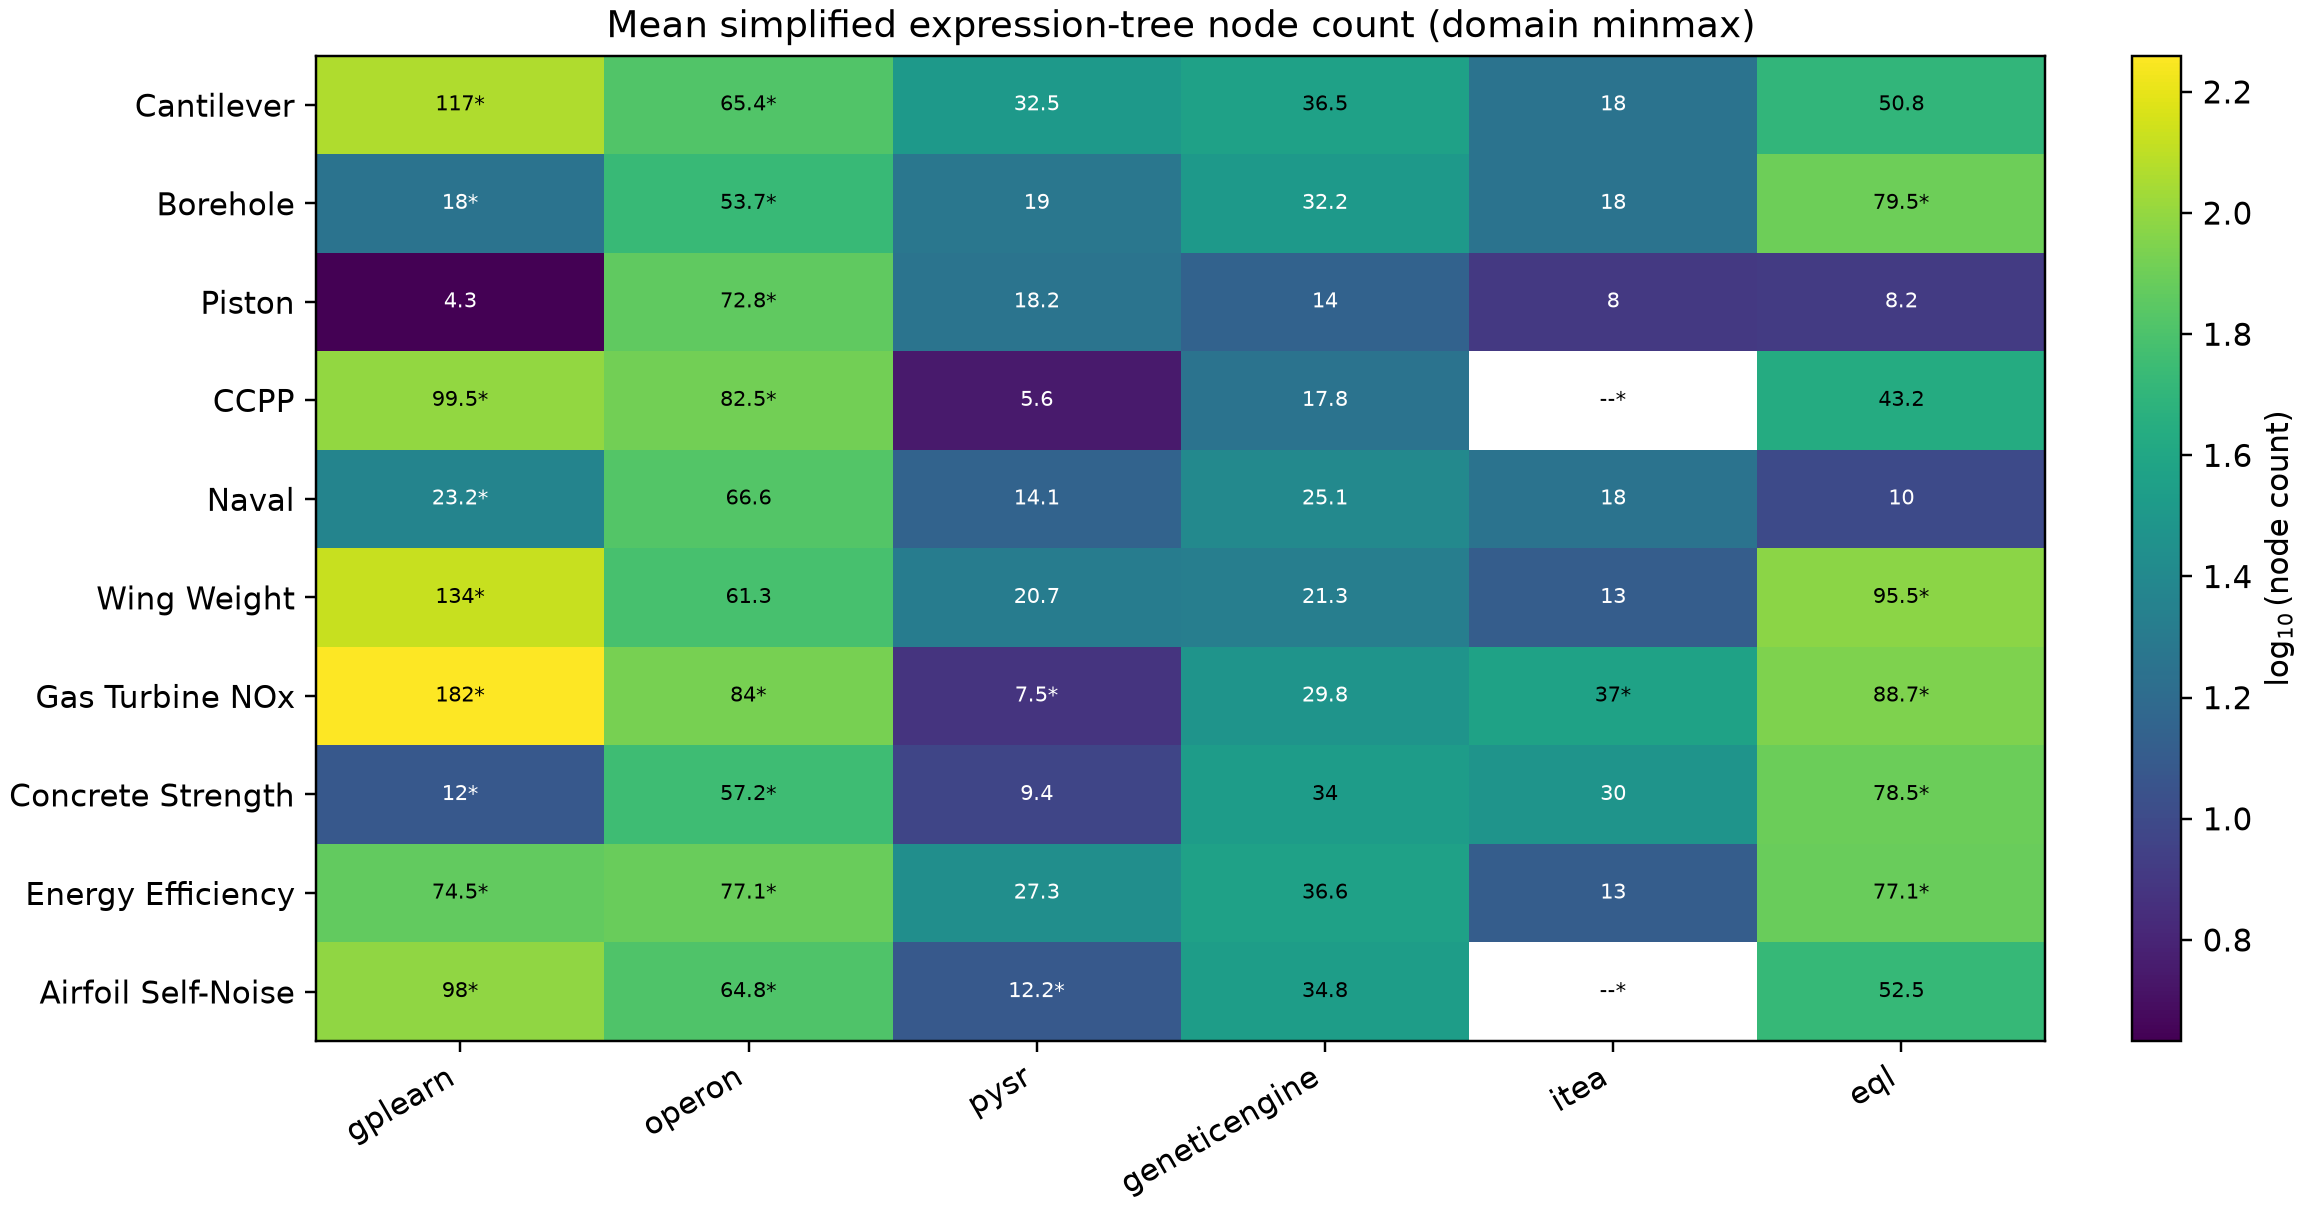
\includegraphics[width=0.96\textwidth]{images/results/complexity_heatmap_domain_minmax.png}
    \caption{Mean simplified expression-tree node count by framework and problem using domain-normalized inputs. An asterisk indicates that at least one expression in the cell required the unsimplified complexity fallback and was excluded from the displayed simplified mean.}
    \label{fig:results-complexity-domain}
\end{figure}

\subsection{Symbolic Simplification and Fallbacks}

The simplification completion rate differed markedly between frameworks. GeneticEngine completed simplification for all 200 parsed expressions, and PySR did so for 195 of 200. gplearn required the unsimplified fallback for 74 of its 199 parsed expressions, the largest number among the frameworks. EQL required 43 fallbacks, Operon 34, and ITEA 24. Because fallback expressions can be structurally larger than their simplified counterparts, the primary simplified-complexity comparison excludes them rather than treating the two forms as directly equivalent.

\begin{table}[H]
    \centering
    \caption{Symbolic simplification outcomes for parsed expressions.}
    \label{tab:results-simplification}
    \begin{tabular}{lrrr}
        \toprule
        Framework & Parsed & Simplified & Fallback rate \\
        \midrule
        gplearn & 199 & 125 & 37.2\% \\
        Operon & 199 & 165 & 17.1\% \\
        PySR & 200 & 195 & 2.5\% \\
        GeneticEngine & 200 & 200 & 0.0\% \\
        ITEA & 200 & 176 & 12.0\% \\
        EQL & 200 & 157 & 21.5\% \\
        \bottomrule
    \end{tabular}
\end{table}

These fallback counts reflect the benchmark's bounded post-processing procedure rather than failures of model fitting. Separating the original trial record from its analysis sidecar preserved the fitted equation and predictive results even when parsing or simplification was incomplete.

\section{Computational Efficiency}

Computational efficiency is reported separately for model fitting and for the subsequent use of the fitted model. This distinction is relevant for surrogate modeling because training is performed once per trial, whereas prediction may be repeated many times after an expression has been obtained.

\subsection{Model-Fitting Time}

Model-fitting times describe the evaluated configurations under the common one-thread execution controls; they are not the result of equal wall-clock search budgets. Operon had the lowest median problem-level mean fit time at 3.88 seconds, followed by ITEA at 5.67 seconds. EQL required 24.50 seconds, gplearn 37.62 seconds, GeneticEngine 60.24 seconds, and PySR 89.66 seconds. PySR's fit times were comparatively consistent with the configured fixed search duration, while the other methods showed stronger problem-dependent variation.

\begin{table}[H]
    \centering
    \caption{Median of problem-level mean model-fitting times across both scaling conditions.}
    \label{tab:results-fit-time-summary}
    \begin{tabular}{lr}
        \toprule
        Framework & Fit time (s) \\
        \midrule
        Operon & 3.88 \\
        ITEA & 5.67 \\
        EQL & 24.50 \\
        gplearn & 37.62 \\
        GeneticEngine & 60.24 \\
        PySR & 89.66 \\
        \bottomrule
    \end{tabular}
\end{table}

Figures~\ref{fig:results-fit-time-raw} and~\ref{fig:results-fit-time-domain} display the problem-level mean fit times separately for raw and normalized inputs. This placement makes it possible to distinguish framework-wide timing differences from problem-specific increases and from the reduced number of successful repetitions in failed configurations.

\begin{figure}[H]
    \centering
    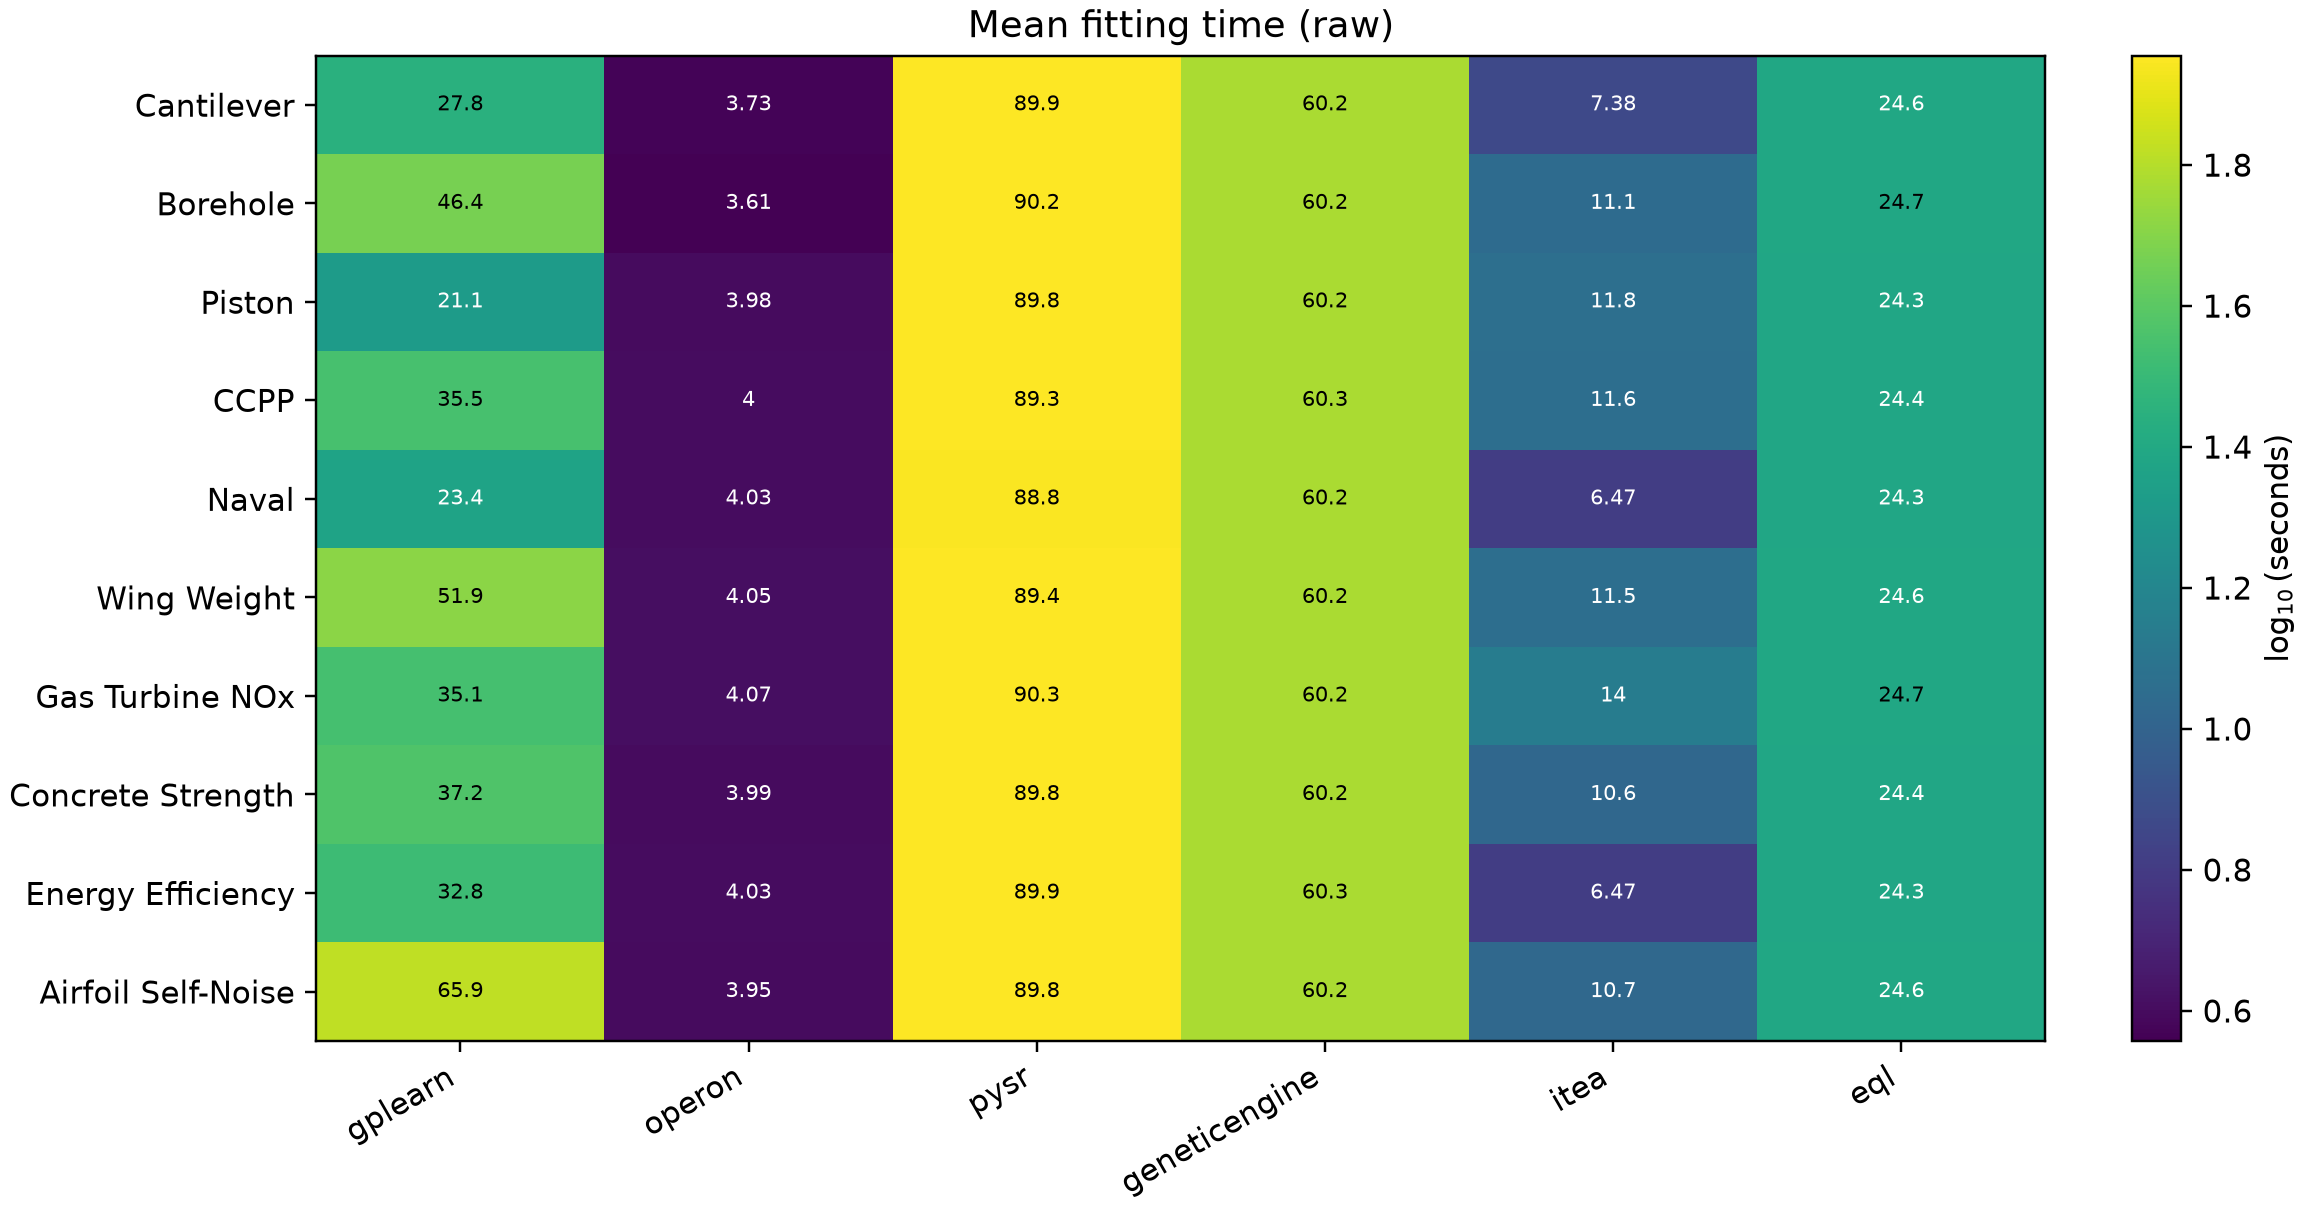
\includegraphics[width=0.96\textwidth]{images/results/fit_time_heatmap_raw.png}
    \caption{Mean model-fitting time by framework and problem using raw inputs. Cell colors represent the base-10 logarithm of time, while annotations report seconds.}
    \label{fig:results-fit-time-raw}
\end{figure}

\begin{figure}[H]
    \centering
    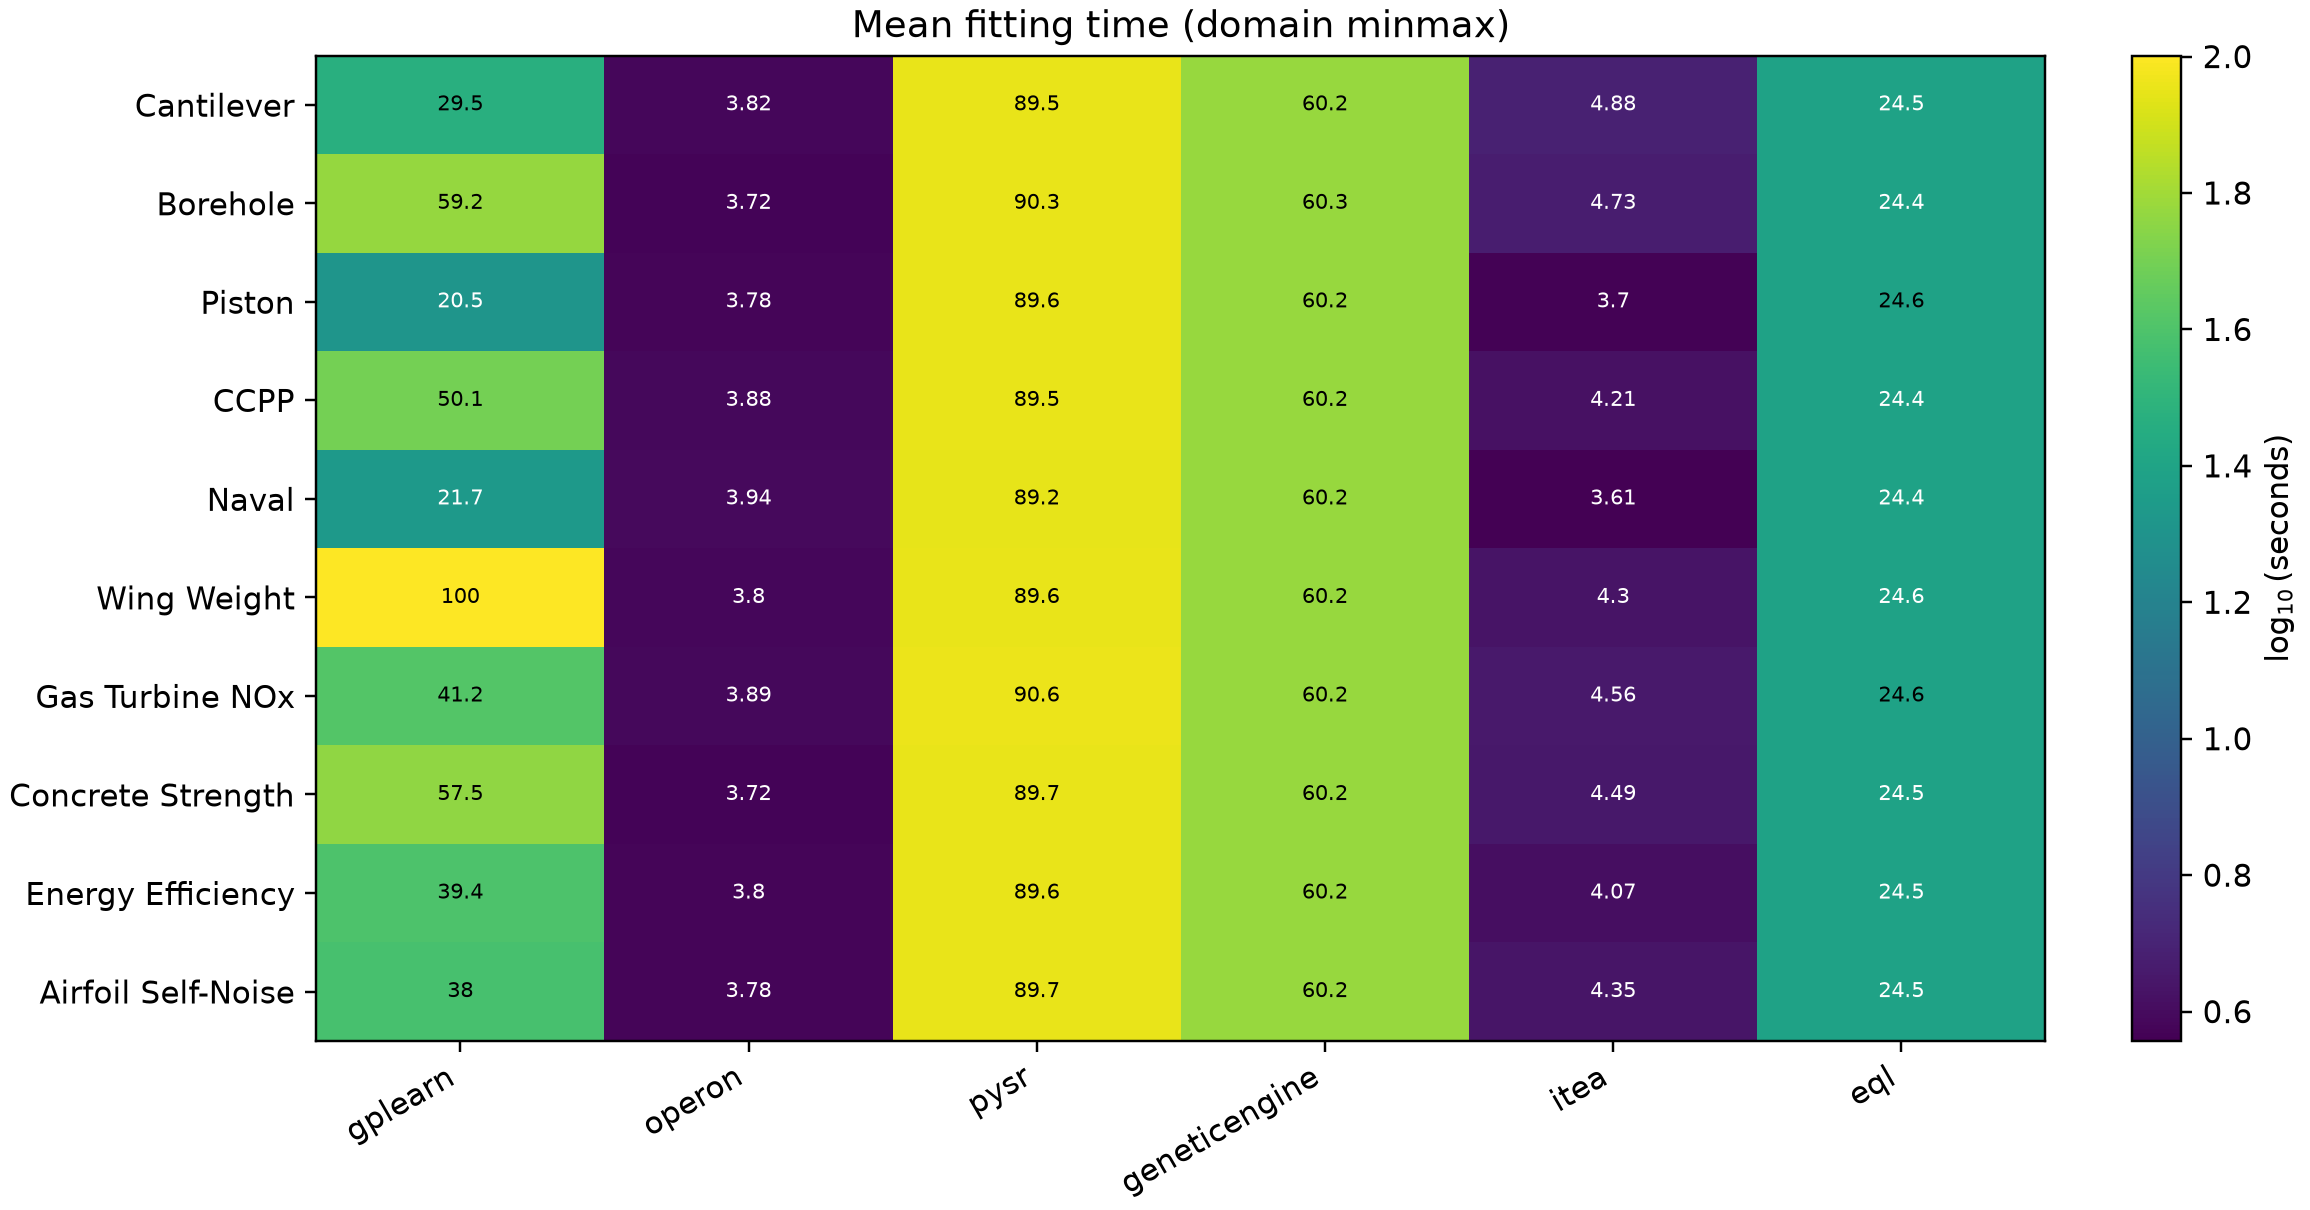
\includegraphics[width=0.96\textwidth]{images/results/fit_time_heatmap_domain_minmax.png}
    \caption{Mean model-fitting time by framework and problem using domain-normalized inputs. Cell colors represent the base-10 logarithm of time, while annotations report seconds and are based on successful trials only.}
    \label{fig:results-fit-time-domain}
\end{figure}

\subsection{Prediction and Expression-Extraction Time}

Prediction was fast for all fitted symbolic models relative to model fitting. Table~\ref{tab:results-prediction-extraction-time} reports medians of the problem-level mean measurements for each scaling condition. Operon and GeneticEngine had the lowest prediction time per observation, while EQL had the highest. Expression extraction was negligible for gplearn, Operon, GeneticEngine, and ITEA, remained below approximately 0.011 seconds for PySR, and required approximately 0.10 seconds for EQL.

\begin{table}[H]
    \centering
    \caption{Median problem-level mean prediction and expression-extraction times. Prediction time is the median full-test prediction duration divided by the number of reference-test observations.}
    \label{tab:results-prediction-extraction-time}
    \begin{tabular}{llrr}
        \toprule
        Framework & Scaling & Prediction ($\mu$s/sample) & Extraction (s) \\
        \midrule
        gplearn & Raw & 0.952 & 0.000294 \\
        gplearn & Domain-normalized & 0.886 & 0.000272 \\
        Operon & Raw & 0.025 & 0.000066 \\
        Operon & Domain-normalized & 0.028 & 0.000064 \\
        PySR & Raw & 0.713 & 0.008723 \\
        PySR & Domain-normalized & 0.852 & 0.010874 \\
        GeneticEngine & Raw & 0.039 & 0.000025 \\
        GeneticEngine & Domain-normalized & 0.040 & 0.000025 \\
        ITEA & Raw & 0.219 & 0.000054 \\
        ITEA & Domain-normalized & 0.231 & 0.000048 \\
        EQL & Raw & 1.915 & 0.096072 \\
        EQL & Domain-normalized & 1.901 & 0.104759 \\
        \bottomrule
    \end{tabular}
\end{table}

Even the largest median prediction time remained below two microseconds per reference-test observation. The fitted expressions were therefore inexpensive to evaluate once training had completed, although the measurements exclude calling-process and container-startup overhead and should be interpreted as in-process prediction costs.

\section{Consolidated Framework Comparison}

Table~\ref{tab:results-consolidated} combines the main framework-level outcomes. Operon provided the strongest overall predictive performance and the shortest model-fitting time, but its expressions were larger than those returned by PySR, ITEA, and GeneticEngine. PySR produced the smallest expressions and completed every trial, at the cost of the longest fitting time. ITEA combined the second-lowest median NRMSE with short fitting times and relatively compact expressions. gplearn completed every trial but was less accurate and produced the largest expressions in the aggregate. GeneticEngine returned compact expressions and completed all trials after its later compatible reruns were incorporated. EQL benefited most consistently from domain normalization and won two normalized analytical configurations, but its aggregate raw-input performance and variability were poor.

\begin{table}[H]
    \centering
    \caption{Consolidated framework comparison. Predictive, timing, and complexity values are medians of problem-level means across both scaling conditions. Simplified node counts exclude fallback expressions.}
    \label{tab:results-consolidated}
    \begin{tabular}{lrrrrr}
        \toprule
        Framework & NRMSE & $R^2$ & Fit time (s) & Nodes & Failed \\
        \midrule
        gplearn & 0.1267 & 0.5064 & 37.62 & 108.39 & 0 \\
        Operon & 0.0259 & 0.9849 & 3.88 & 66.00 & 1 \\
        PySR & 0.0773 & 0.8396 & 89.66 & 11.21 & 0 \\
        GeneticEngine & 0.1187 & 0.6101 & 60.24 & 26.10 & 0 \\
        ITEA & 0.0722 & 0.8564 & 5.67 & 21.60 & 0 \\
        EQL & 0.1791 & -0.5483 & 24.50 & 51.65 & 0 \\
        \bottomrule
    \end{tabular}
\end{table}

The results do not identify one framework as best under every evaluation dimension. Operon dominated the predictive and fitting-time summaries, PySR minimized syntactic expression size, ITEA offered a strong balance of accuracy, speed, and compactness, and EQL demonstrated the clearest dependence on input scaling. These observed trade-offs, together with the variation in symbolic-analysis coverage and the single unresolved execution failure, form the basis of the interpretation in the following chapter.


\chapter{Discussion}

This chapter interprets the benchmark results in relation to the research question and the intended use of Symbolic Regression for surrogate modeling. The comparison does not support a single ranking that is valid for every application. Instead, it reveals trade-offs between predictive accuracy, expression size, computational effort, stability, preprocessing requirements, and practical reliability. The implications of these trade-offs are discussed first, followed by an assessment of the suitability of the evaluated frameworks and the limitations and research needs exposed by the benchmark.

\section{Interpretation of Framework Trade-Offs}

The clearest overall result is the strong performance of Operon under the evaluated configuration. It achieved the lowest mean NRMSE in 13 of the 20 problem--scaling combinations, the best median predictive performance, and the shortest median fitting time. This combination shows that evolutionary symbolic regression does not necessarily require a choice between good prediction and practical execution time. However, Operon's median simplified expression size of 66 nodes was substantially larger than those of PySR, ITEA, and GeneticEngine. Its advantage therefore concerns prediction and computational efficiency more clearly than equation compactness. The remaining failed trial also belonged to Operon, although one failure among 200 assigned trials does not change its otherwise high execution coverage.

PySR displayed a different profile. Its median predictive performance was weaker than that of Operon and ITEA, and its configured fitting time was the longest among the six frameworks. At the same time, it returned the smallest expressions by a considerable margin and completed all assigned trials. This makes PySR relevant when compact symbolic output is valued more strongly than fitting time or the lowest aggregate error. The result also illustrates why accuracy and complexity should be reported separately: selecting a framework only from the predictive ranking would overlook PySR's main advantage, while selecting only from expression size would conceal its computational cost and weaker performance on several problems.

ITEA provided the most balanced aggregate profile after Operon. It achieved the second-lowest median NRMSE, short fitting times, and comparatively compact expressions. It was also the strongest method on both CCPP conditions and on raw Airfoil Self-Noise. Its extremely small variation across repetitions must nevertheless be interpreted cautiously because the employed adapter does not expose a controllable estimator seed. The repeated results demonstrate stable behavior when the same implementation is invoked repeatedly, but they do not establish seed-controlled reproducibility in the same sense as for frameworks that accept the configured repetition labels.

The remaining frameworks showed more pronounced limitations. gplearn provided a dependable conventional genetic-programming reference and completed every trial, but it produced the largest expressions and did not lead any problem--scaling combination. GeneticEngine also completed all trials after the scalar-prediction compatibility issue was handled, and its equations were relatively compact, but its aggregate predictive performance was below that of Operon, ITEA, and PySR. EQL achieved the best normalized-input result on Borehole and Wing Weight, demonstrating that its differentiable representation can be effective on suitable analytical structures. Its raw-input results, however, contained severe errors and high repetition variability. EQL therefore provided the clearest example of a framework whose usefulness depends on preprocessing rather than being an invariant property of the method.

The normalization experiment confirms that input scaling cannot be treated as a universally beneficial preprocessing step. Domain normalization improved EQL on every problem and improved PySR on six, but it improved gplearn, GeneticEngine, and ITEA on only two problems each. Operon's median error was almost unchanged. For EQL, normalization largely prevented extreme raw-input behavior, whereas for several evolutionary methods it sometimes increased error. The practical implication is that scaling should be treated as part of a framework configuration and reported explicitly. A comparison based on only one input representation could favor or disadvantage particular method families without making that dependence visible.

Problem characteristics were at least as important as the framework choice. The analytical problems generally permitted lower errors than the empirical datasets, but no method was consistently strongest on every analytical expression. Among the external problems, Energy Efficiency was approximated comparatively well, while Gas Turbine NOx remained difficult for all frameworks and produced negative mean $R^2$ even for the best method. This variation supports the observation from broader SR benchmarks that no single approach is uniformly optimal across problem classes \cite{lacava2021contemporary,dong2025recent}. It also cautions against drawing general conclusions from a small number of favorable analytical examples.

Runtime results require a similarly bounded interpretation. Operon and ITEA were fastest under the selected configurations, but the benchmark did not impose equal wall-clock or function-evaluation budgets. PySR and GeneticEngine were explicitly constrained by practical time budgets, while the other frameworks used their adapter-specific iteration or evaluation controls. The measured times therefore describe the cost and outcome of the configurations actually evaluated, not the maximum attainable performance of each framework or an equal-compute competition. Nevertheless, the very low prediction times of all returned expressions demonstrate a shared advantage after fitting: every successful symbolic surrogate could be evaluated in microseconds per sample, making repeated deployment inexpensive compared with the search process.

\section{Suitability for Interpretable Surrogate Modeling}

The benchmark supports Symbolic Regression as a useful but conditional approach to interpretable surrogate modeling. The evaluated frameworks produced explicit expressions for almost every successful trial, and these expressions could usually be parsed, transformed into physical input coordinates, and assigned common structural measures. Once fitted, the models were inexpensive to evaluate. These properties make SR suitable when an application requires a reusable analytical surrogate whose variables and operations can be inspected directly rather than a prediction interface alone.

Explicitness, however, should not be equated automatically with interpretability. The median simplified expressions ranged from approximately 11 nodes for PySR to more than 108 nodes for gplearn, and individual problem-level means were considerably larger. An equation with many nested operations can be technically visible while remaining difficult to understand. Node count is also only a syntactic proxy: it does not measure whether the variables have physically plausible roles, whether constants correspond to meaningful quantities, or whether the expression communicates a useful scientific relationship. The simplification fallbacks reinforce this distinction because 180 parsed expressions could not be reduced within the bounded procedure and were therefore excluded from the primary simplified-complexity means.

The structural statistics must also be considered together with predictive adequacy. The negative $R^2$ results on Gas Turbine NOx show that an inspectable equation is not useful as a surrogate merely because it is symbolic. Conversely, the stronger Energy Efficiency, CCPP, Naval Propulsion, Concrete Strength, and Airfoil Self-Noise results show that SR can provide workable approximations for several engineering datasets under modest training sizes. Whether those expressions are scientifically informative would require domain-specific review beyond the structural measures used here.

The framework choice should consequently follow the intended use. Operon is the strongest candidate from this benchmark when predictive accuracy and fitting speed are primary, provided that moderately larger expressions are acceptable. PySR is preferable when compact output is a central requirement and longer fitting time is tolerable. ITEA offers a favorable compromise between accuracy, speed, and expression size, although its uncontrolled repetition behavior should be considered when strict seed reproducibility is required. EQL may be useful for compatible analytical structures but should be used with normalized inputs and careful stability checks. gplearn remains useful as a transparent conventional baseline, while GeneticEngine offers compact grammar-guided models but did not match the leading predictive results in this configuration.

Practical suitability also depends on the surrounding software rather than the search algorithm alone. The benchmark required pinned containers, adapter-specific compatibility handling, explicit failure records, and separate symbolic post-processing. The GeneticEngine scalar-output issue demonstrated that a valid constant phenotype can appear to be a failed trial when framework output conventions are not harmonized. The final resolved matrix achieved 1199 successful trials out of 1200, indicating that the selected tools can be integrated reliably, but only after such interface differences are made explicit. Reproducible surrogate modeling therefore requires preservation of configurations, environments, data hashes, expressions, and post-processing decisions in addition to the equation returned by the framework.

Taken together, the answer to the research question is qualified. Current SR frameworks are suitable for constructing inexpensive and inspectable surrogate models on a range of scientific and engineering regression tasks, but suitability is problem- and objective-dependent. The benchmark does not support treating SR as an automatic route to simple or scientifically correct equations. Its main value is the ability to expose the predictive model in mathematical form while allowing accuracy, complexity, and domain plausibility to be evaluated together.

\section{Research Gaps and Future Benchmarking Needs}

Several limitations define the scope of these conclusions. The benchmark contains ten problems and uses one fixed training and reference-test design for each. Although the collection includes analytical, simulator-generated, experimental, and measured data, it is not large enough to represent the full diversity of surrogate-modeling applications. The conclusions are therefore evidence about the evaluated tasks and configurations rather than population-wide rankings of SR frameworks. Future work should extend the collection with additional dimensionalities, sample sizes, noise levels, discontinuities, and domain structures while retaining transparent dataset provenance.

The experimental protocol evaluates interpolation on held-out observations but does not directly test extrapolation beyond the documented training region, sensitivity to corrupted measurements, or stability during recursive simulation. These properties are important when a surrogate replaces a scientific simulator or is used in optimization and control. Future benchmark tracks should distinguish interpolation from controlled extrapolation, add repeated noise conditions, and include dynamical rollout tasks where prediction errors can accumulate. Physical constraints such as dimensional consistency, monotonicity, conservation relationships, and admissible output ranges should also be tested when the problem supplies them.

The comparison uses one fixed configuration per framework and deliberately avoids tuning on the test results. This supports reproducibility but leaves open how much each method would benefit from problem-specific operator sets, complexity penalties, or search budgets. A stronger future comparison could define both a common wall-clock track and a framework-specific recommended-configuration track. Accuracy--complexity Pareto fronts should be retained rather than reducing each run to one selected expression, because different applications may prefer different points on that frontier. Reporting memory consumption and energy use would further improve the computational comparison advocated in recent work on more comprehensive SR evaluation \cite{defranca2025srbench,aldeia2025call}.

The absence of non-symbolic baselines limits conclusions about whether SR pays an accuracy cost for explicitness. Including linear and polynomial regression, gradient-boosted trees, Gaussian processes, and compact neural networks under the same data splits would show when symbolic models are competitive with established surrogate methods. Such a comparison should not use predictive error alone: model-evaluation cost, calibration, uncertainty estimates, and the availability and faithfulness of explanations would provide a more meaningful reference for the benefits claimed by intrinsically interpretable models.

Interpretability itself requires broader evaluation. This thesis measures expression size, depth, operators, constants, and variables, but these quantities do not fully capture human understanding. Future studies should combine syntactic measures with expert assessment of physical plausibility, dimensional validity, recognizable substructures, and the effort required to explain an equation. Controlled user studies could test whether scientists or engineers actually make better judgments with the returned symbolic models. The distinction between a small expression and a meaningful expression is especially important when simplification introduces numerically fitted constants or algebraically unusual but compact forms.

Finally, the benchmark exposed the importance of infrastructure as a research topic. Framework APIs, expression languages, random-seed controls, and prediction shapes remain inconsistent. Common schemas for expressions, protected operators, complexity, resource budgets, and failure reporting would reduce the amount of adapter-specific logic and make independent reproduction easier. The coordinate-level newest-compatible-result resolver introduced for this thesis also illustrates why provenance must be maintained when benchmark suites evolve: later reruns should be incorporated without silently mixing incompatible protocols. Continued development toward standardized, versioned, and auditable SR benchmarks is therefore necessary for reliable comparison and practical adoption.


\chapter{Conclusion}

This chapter summarizes the principal findings, answers the research question, and identifies the most important directions for extending the benchmark. The conclusions apply to the evaluated datasets, framework versions, and fixed configurations and should not be interpreted as universal rankings of Symbolic Regression methods.

\section{Summary of Findings}

The benchmark compared gplearn, Operon, PySR, GeneticEngine, ITEA, and EQL on ten analytical, simulator-generated, experimental, and measured surrogate-modeling problems. Each framework was evaluated with raw and domain-normalized inputs over ten repetitions, producing 1200 planned trial coordinates. Of these, 1199 completed successfully, and all successful trials received a current symbolic-analysis record. A common protocol, fixed train--test tables, pinned container images, configuration hashes, and coordinate-level result resolution were used to preserve comparability and traceability as the problem collection was expanded.

Operon achieved the strongest overall predictive result under the evaluated configurations. It obtained the lowest mean range-normalized RMSE in 13 of the 20 problem--scaling combinations, the lowest median value of 0.0259, and the shortest median fitting time of 3.88 seconds. ITEA provided a strong compromise, combining the second-lowest median error with short fitting times and relatively compact expressions, although its adapter did not expose a controllable repetition seed. PySR produced the smallest expressions, with a median problem-level mean of approximately 11 simplified nodes, but also had the longest median fitting time. gplearn was reliable but produced the largest expressions, GeneticEngine returned comparatively compact models but weaker predictive results, and EQL showed the greatest dependence on input normalization.

The experiments also showed that preprocessing and problem characteristics can substantially affect the apparent quality of a framework. Domain normalization improved EQL on every problem but was not consistently beneficial for the evolutionary methods. Gas Turbine NOx remained difficult for all frameworks, whereas several analytical problems and the Energy Efficiency dataset admitted substantially lower prediction errors. Repetition variability likewise differed between frameworks and scaling conditions. Once fitted, however, the symbolic surrogates were inexpensive to evaluate: at the framework-summary level, median prediction costs remained below two microseconds per test observation.

Expression structure introduced a separate trade-off from predictive accuracy. Smaller expressions were not always the most accurate, and the framework with the strongest predictive performance did not produce the smallest models. Most returned expressions could be parsed and measured through the common SymPy representation, but simplification required an unsimplified fallback for 180 expressions. These results support reporting structural coverage and complexity alongside accuracy rather than treating the availability of an explicit equation as sufficient evidence of interpretability.

\section{Answer to the Research Question}

The results support Symbolic Regression as a suitable approach for constructing inexpensive and inspectable surrogate models, but only with important qualifications. The evaluated frameworks usually produced explicit expressions that could be extracted, parsed, structurally analyzed, and evaluated at low cost. This makes SR useful when a surrogate must support repeated prediction while also exposing its variables and mathematical operations for inspection.

Suitability nevertheless depends on the problem and the objective of the application. Operon is the strongest candidate in this benchmark when predictive accuracy and fitting speed are prioritized and moderately larger expressions are acceptable. PySR is more appropriate when compact symbolic output is central and longer fitting time can be tolerated. ITEA offers a favorable balance of predictive performance, runtime, and expression size, while EQL requires particular attention to input scaling and stability. gplearn provides a conventional and dependable baseline, and GeneticEngine offers relatively compact grammar-guided expressions but did not match the leading predictive results under the selected configuration.

Predictive success alone does not guarantee that a symbolic model is simple, stable across repetitions, physically plausible, or scientifically correct. Conversely, a compact expression is not useful as a surrogate if its predictions are inadequate. The structural statistics used in this thesis measure syntactic inspectability rather than human understanding or domain validity. SR should therefore be treated as a way to expose a predictive model in mathematical form, after which accuracy, complexity, stability, and application-specific plausibility must be assessed together.

Practical usability also depends on the surrounding software workflow. The near-complete trial matrix demonstrates that all six frameworks can be integrated successfully, but this required pinned containers, common prediction-shape handling, adapter-specific compatibility logic, explicit failure reporting, and separate symbolic post-processing. Seed control, expression-export behavior, parsing coverage, and environment reproducibility are consequently part of a framework's suitability, not merely implementation details separate from the algorithm.

\section{Outlook and Future Work}

Future evaluations should extend the problem collection while preserving the fixed, auditable protocol. Additional tasks should cover larger sample sizes, higher dimensions, discontinuities, controlled noise, and application-specific physical constraints. Separate interpolation and extrapolation tracks would reveal whether expressions that perform well inside the sampled domain remain reliable outside it, while dynamical rollout experiments could assess error accumulation during repeated use.

The comparison could also be strengthened through non-symbolic surrogate baselines and complementary budget tracks. Linear and polynomial regression, Gaussian processes, tree ensembles, and compact neural networks would provide context for the predictive cost of obtaining an explicit expression. A common wall-clock track could complement the present fixed framework configurations, while framework-specific recommended settings and complete accuracy--complexity Pareto fronts would show how sensitive the conclusions are to search budgets and model selection.

Finally, interpretability should be evaluated beyond syntactic complexity. Domain experts could assess dimensional consistency, physical plausibility, recognizable interactions, and the effort required to understand or validate an expression. At the infrastructure level, more consistent framework interfaces for seed control, protected operators, expression export, complexity definitions, and failure diagnostics would reduce adapter-specific work and improve independent reproduction. These extensions would provide a stronger basis for deciding when an explicit symbolic surrogate offers a practical advantage over established alternatives.

%
% agsm in der uibk vorlage
%
% ^.

\bibliographystyle{agsm} %apalike
\bibliography{literatur}


\end{document}
